\documentclass[12pt,a4paper]{article}
\usepackage{graphicx, float}
\usepackage[round]{natbib}
\usepackage{enumitem}
\usepackage{tabularx}
\usepackage[hidelinks]{hyperref}
\usepackage{booktabs}
\usepackage{array}
\usepackage{multirow}
\usepackage{xcolor}
\usepackage{xurl}
\usepackage{amsmath}
\usepackage{amssymb}
\usepackage{tikz}
\usepackage{helvet}
\usepackage{geometry}
\geometry{margin=2.5cm}
\renewcommand{\arraystretch}{1.25}
\graphicspath{{images/}}

\bibliographystyle{apalike}

\title{From Competition to Cooperation:\\Teaching LLMs Pareto-Efficient Negotiation with LA-GRPO}
\author{Michael Gubler}
\date{May 2026}

\begin{document}

% ============================================================
% TITLE PAGE
% ============================================================
\begin{titlepage}
    \thispagestyle{empty}
    \centering

    {\LARGE \textbf{From Competition to Cooperation}\par}
    \vspace{0.4cm}
    {\large \textbf{Teaching LLMs Pareto-Efficient Negotiation with LA-GRPO}\par}
    \vspace{0.6cm}
    {\large \textbf{Master Thesis}\par}

    \vspace{1.5cm}

    \begin{flushleft}
    \begin{tabular}{@{}l p{9cm}@{}}
        \textbf{Author:} & Michael Gubler \\
                         & Dättnauerstrasse 133 \\
                         & CH-8406 Winterthur \\
                         & michael.gubler@stud.hslu.ch \\[1.0em]

        \textbf{Supervisor:} & Oliver Staubli \\
                             & Lucerne University of Applied Sciences and Arts \\
                             & Werftestrasse 4 \\
                             & CH-6002 Lucerne \\
                             & oliver.staubli@hslu.ch \\[1.0em]

        \textbf{Co-Supervisor:} & Peter Niederberger \\
                                & Tincan AG \\
                                & Feldpark 17 \\
                                & CH-6300 Zug \\
                                & p.niederberger@tincan.ch \\
    \end{tabular}
    \end{flushleft}

    \vfill

    \centering
    Lucerne University of Applied Sciences and Arts \\[0.2cm]
    \textbf{Master of Science in Applied Information and Data Science (MScIDS)} \\[0.2cm]
    Spring Semester 2026 \\[1.2cm]

    Winterthur, May 2026
\end{titlepage}

\newpage
\tableofcontents
\newpage


% ============================================================
% 1. INTRODUCTION
% ============================================================
\section{Introduction}
\label{sec:introduction}

Large Language Models (LLMs) have rapidly advanced in their ability to conduct multi-turn dialogues across a variety of domains, ranging from tutoring and healthcare to code generation and strategic interaction. A particularly relevant testbed for studying multi-turn reasoning is negotiation, where agents must balance short-term concessions with long-term gains, maintain coherence across multiple exchanges, and adapt to dynamic counterpart behavior. For instance, GPT-4 and similar models already perform well on various negotiation subtasks (e.g. understanding offers and devising counter-proposals), often matching or surpassing specialized models in objective evaluations \citep{kwon-etal-2024-llms}. 
\par
\citet{franceschetti2025advantage} introduced Local Advantage Group Relative Policy Optimization (LA-GRPO), a novel method that addresses the credit assignment problem in multi-turn dialogues by isolating learning signals at the turn level. LA-GRPO outperformed traditional GRPO in complex bargaining settings, achieving more efficient and effective negotiation strategies without degrading general language capabilities. However, this work primarily focused on zero-sum bargaining scenarios, where one party's gain directly translates into the other's loss.
\par
While zero-sum games are analytically convenient, many real-world negotiations are non-zero-sum. Examples include labor agreements, international treaties, or business partnerships, where cooperation and joint value creation play a critical role. In such contexts, success is not only measured by maximizing individual payoff but also by achieving Pareto-efficient outcomes, where no party can be made better off without making the other worse off. Cooperative negotiation requires LLMs to balance self-interest with fairness, recognize opportunities for mutual gain, and avoid exploitative strategies that may undermine long-term trust or stability.
\par
Most existing research and alignment of LLM-based negotiators has focused on competitive or zero-sum settings. \citet{jiang-akcakir-2025-explicit} noted that in the absence of explicit negotiation instructions, LLMs showed a 50-90\% lower success rate than in instructed scenarios. In other words, current LLMs are trained to compete for the largest share, with little attention to fairness or joint outcomes. Human negotiation theory warns of a ``negotiator's dilemma,'' where tactics for claiming value (hard bargaining and withholding information) directly undermine those for creating value (open sharing and building trust). If both parties compete relentlessly, the result is often a dead end or a mediocre compromise, whereas mutual cooperation could have yielded a better Pareto-optimal outcome \citep{lax1992manager_summary}. Notably, a recent AI negotiation competition found that agents using warm and cooperative communication achieved higher joint gains and more agreements, whereas overly dominant agents frequently stalemated \citep{vaccaro2025advancingainegotiationsnew}.
\par
As AI negotiators are expected to enter the real world en masse in the near future, it is important to increase value creation for everyone by training LLMs to both compete and cooperate intuitively -- without the need of explicit prior instructions.


\subsection{Thematic Scope}

This thesis builds directly on \citeauthor{franceschetti2025advantage}'s (\citeyear{franceschetti2025advantage}) work by shifting the focus from competition to cooperation. It investigates how LA-GRPO and related alignment techniques can be adapted to multi-objective reward structures, enabling LLMs to learn negotiation strategies that maximize both individual and collective outcomes. This requires agents to identify creative trade-offs and integrative solutions that improve overall welfare for everyone. The overarching aim is to investigate whether alignment methods originally developed for zero-sum bargaining can be adapted to teach models cooperative behavior - balancing self-interest with collective welfare.
\par
The thematic emphasis on cooperation is not only of academic interest but carries significant real-world relevance. Many of the most pressing negotiation challenges in society are fundamentally non-zero-sum. For example contract negotiations in business benefit from collaborative thinking: long-term partnerships flourish when agreements are seen as fair and value-maximizing for both client and provider, rather than one party squeezing the other.
\par
A central aspect of this exploration is the learning process itself. Franceschetti's thesis showed that applying credit assignment locally at the dialogue-turn level led to more stable and efficient learning in competitive negotiations. Building on that insight, this work examines whether similar turn-level learning dynamics can foster cooperation and therefore allowing the model to recognize the consequences of individual utterances and gradually internalize strategies that promote mutual gain.
\par
The thesis employs multi-issue negotiation tasks as test environments. Unlike a simple single-issue deal where one side's gain equals the other's loss, multi-issue negotiations allow for trade-offs that benefit both sides. Examples include the Nash Bargaining Game and the Two-Issue Bargaining Problem, which will be explained further in the next chapter.
\par
Finally, cooperation must of course be tempered with robustness to defection. In practice, a negotiator (whether human or AI) should be willing to cooperate but not naïvely so---it should remain effective if the other side attempts to use aggressive or manipulative tactics. A subtler aspect of the thesis's scope is therefore to explore whether cooperative agents maintain their negotiation performance when facing adversarial counterparts, rather than collapsing into either exploitation or unproductive resistance. This balance between collaboration and robustness is critical for real-world deployment: it mirrors the way effective human negotiators build trust and find common ground, while still holding firm against bad-faith partners.


\subsection{Research Questions}
To that end, the following key research questions are investigated:

\begin{enumerate}[label={}, leftmargin=0pt, itemsep=1.2em]
    \item \textbf{RQ1: Turn-Level Learning:} Does applying LA-GRPO at the single-turn level improve learning performance in cooperative negotiation games?
    \par This question tests whether applying LA-GRPO at the single-turn level improves negotiation outcomes compared to baseline GRPO. The two methods are compared on three key metrics (agreement rate, agent payoff $U_A$, Nash product) in two ways: once at the end of training (full convergence), and once at the same compute budget. This makes it possible to separate the effect of the method itself from the effect of longer training.

    \item \textbf{RQ2: Reward Function Design:} How can reward functions be designed to balance individual payoff maximization with collective welfare and fairness?
    \par This question looks at how different ways of combining reward components affect negotiation results. Five reward setups are tested by varying the weights ($\lambda$ parameters) on self-interest, social welfare, and fairness. A good setup produces high joint value and balanced outcomes without making the agent's own payoff much worse.

    \item \textbf{RQ3: Cooperation-Focused Metrics:} Which evaluation metrics best capture cooperative success in negotiation beyond traditional utility scores?
    \par This question examines which evaluation metrics best capture cooperative behavior. In addition to individual utility ($U_A$), outcomes are assessed using social welfare ($U_A + U_B$), Nash product ($U_A \times U_B$), and game-normalized ratios that enable comparison across heterogeneous game configurations. Scatter plots of $U_A$ vs.\ $U_B$ are used to visualize the distribution of negotiation outcomes relative to the equal-payoff diagonal.

    \item \textbf{RQ4: Robustness to Defection:} Can LLMs trained for cooperation maintain robustness and negotiation effectiveness when facing non-cooperative or adversarial counterparts?
    \par This question tests whether cooperative agents stay effective when the other side plays unfairly. The trained model is evaluated against four adversarial opponent types that each use a different tactic: \emph{hardball} (refuses to give in and stays aggressive), \emph{deceptive} (lies about its own preferences), \emph{anchoring} (starts with an extreme offer to bias the negotiation), and \emph{stubborn} (never compromises regardless of the situation).

    \item \textbf{RQ5: Impact on LLM Capabilities:} To what extent does promoting cooperation affect the linguistic and reasoning capabilities of the underlying LLM?
    \par This question evaluates whether training for cooperation affects general reasoning and instruction-following ability. The fine-tuned models are tested on standard benchmarks covering academic knowledge (MMLU-Pro), instruction following (IFEval), and mathematical reasoning (GSM8K), and compared to the base model to detect possible capability loss.
\end{enumerate}


\subsection{Thesis Structure}
The remainder of this thesis is organized as follows. Chapter~\ref{sec:background} provides the theoretical background on negotiation theory, cooperative game theory, and reinforcement learning alignment methods. Chapter~\ref{sec:methodology} describes the methodological contribution---adapting LA-GRPO for cooperative reward signals. Chapter~\ref{sec:experimental_setup} details the experimental setup, including the negotiation environment, game design, and evaluation pipeline. Chapter~\ref{sec:results} presents and discusses the results. Chapter~\ref{sec:conclusion} concludes with a summary, limitations, and future directions.


% ============================================================
% 2. THEORETICAL BACKGROUND AND RELATED WORK
% ============================================================
\newpage
\section{Theoretical Background and Related Work}
\label{sec:background}

This chapter provides the conceptual foundation for the thesis. It connects negotiation theory, cooperative game theory, and reinforcement learning alignment, and identifies the limitations of current methods in promoting cooperation.

\subsection{Negotiations as Multi-Agent Decision Processes}

Franceschetti formulated multi-turn negotiation as a Markov Decision Process (MDP), where states $s_t$ correspond to the dialogue history of utterances $\{u_0, u_1, \ldots, u_{t-1}\}$ exchanged up to turn $t$, actions $a_t$ represent the next utterance $u_t$, and a terminal reward $R(s_N)$ is assigned at the end of the negotiation based on the agreed outcome. Two agents alternate offers over $N=5$ rounds each, following an alternating-offer protocol. The agent's payoff is denoted $U_A$ and the opponent's payoff $U_B$; both are computed from the issue values agreed upon at the end of the negotiation.

Formally, the negotiation is defined as a tuple $\mathcal{M} = (\mathcal{S}, \mathcal{A}, P, R, \gamma)$:

\begin{itemize}
    \item $\mathcal{S}$: the state space. Each state $s_t$ is the concatenation of the system prompt (scenario description, role description, payoff tables) and the dialogue history $\{u_0, u_1, \ldots, u_{t-1}\}$ up to turn $t$.
    \item $\mathcal{A}$: the action space. An action $a_t = u_t$ is a natural-language utterance generated token-by-token by the policy $\pi_\theta(a_t \mid s_t)$. The utterance itself is a sequence of tokens, making the overall problem a hierarchical generation task.
    \item $P$: the state transition. Transitions are deterministic at the dialogue level: $s_{t+1} = s_t \oplus u_t$, where $\oplus$ denotes appending the utterance to the history. Stochasticity enters only through the opponent's policy $\pi_c$, which is frozen during training.
    \item $R$: the reward function. Intermediate turns yield zero reward; only the terminal state $s_N$ (reached after both agents have had $N$ rounds or a deal has been confirmed) produces a reward $R(s_N)$. The reward is computed from the agreed-upon issue values $(v_1, \ldots, v_K)$ extracted from the dialogue: $R(s_N) = R_{\text{coop}}(U_A, U_B)$ as defined in Section~\ref{sec:cooperative_reward}.
    \item $\gamma \in [0, 1]$: the discount factor, set to $\gamma = 1$ throughout because the only nonzero reward is terminal and the horizon is short and fixed.
\end{itemize}

The objective is to find a policy $\pi_\theta$ that maximizes the expected terminal reward:
\begin{equation}
\max_\theta \; \mathbb{E}_{s_N \sim \pi_\theta, \pi_c} \left[ R_{\text{coop}}(U_A, U_B) \right].
\end{equation}

This formulation treats the entire dialogue as a single episode and is standard for RLHF-style language model training. The token-level policy $\pi_\theta(y_t \mid y_{<t}, s_t)$ that generates each utterance is implicitly embedded in the utterance-level action $a_t = u_t$; GRPO and LA-GRPO compute the loss at the token level, but credit assignment operates at either the full-episode level (GRPO) or the single-turn level (LA-GRPO, see Section~\ref{sec:la_grpo}).

In zero-sum settings, $U_A + U_B$ is approximately constant---one agent's gain is the other's loss. The key departure in this thesis is the extension to \textbf{non-zero-sum} (mixed-motive) games, where $U_A + U_B$ varies across outcomes. In integrative games, trade-offs between issues of differing importance create opportunities for mutual gain that do not exist in purely distributive settings.

\subsection{Cooperative and Integrative Negotiation Theory}\label{sec:cooperative_negotiation_theory}

The theoretical foundation for evaluating cooperative negotiation outcomes rests on three interrelated concepts: Pareto efficiency, the Nash bargaining solution, and integrative bargaining. An outcome is Pareto-efficient if no alternative exists that makes one party better off without making the other worse off. In multi-issue negotiations, Pareto-efficient outcomes typically require agents to identify and exploit differences in issue importance, conceding on less-valued issues in exchange for gains on more-valued ones \citep{lax1992manager_summary}. This mechanism, known as integrative bargaining or log-rolling, distinguishes multi-issue negotiations from single-issue distributive bargaining: rather than simply dividing a fixed pie, agents can create value through package deals that exploit asymmetric preferences.

To select among the many Pareto-efficient outcomes, \citet{Nash1950THEBP} introduced the Nash bargaining solution, which identifies fair and efficient outcomes by maximizing the product of agents' utilities. The Nash product $U_A \times U_B$ is the unique solution satisfying four axioms: Pareto efficiency, symmetry, scale invariance, and independence of irrelevant alternatives. This axiomatic foundation makes the Nash product a theoretically grounded single metric for cooperative success, capturing both efficiency (high total value) and fairness (balanced distribution) in one expression.

A more recent result by \citet{caragiannis2019unreasonable} strengthens the case for the Nash product. They show that in allocation problems, maximizing Nash welfare simultaneously achieves envy-freeness up to one good \emph{and} Pareto efficiency---a property they describe as ``unreasonable'' because Nash welfare was originally designed only for efficiency, yet it also provides strong fairness guarantees. This dual property provides the strongest theoretical argument for using the Nash product as the dominant cooperative term in the reward function of this work: a single, well-motivated metric simultaneously rewards both joint value creation and balanced distribution between the negotiating parties.

\subsection{Alignment Methods for Multi-Turn Dialogue}

\begin{table}[H]
\centering
\caption{Comparison of alignment methods for multi-turn negotiation.}
\label{tab:alignment_methods}
\begin{tabular}{llll}
\toprule
\textbf{Method} & \textbf{Loss} & \textbf{Sampling} & \textbf{Mode} \\
\midrule
DPO & Sigmoid preference & Full trajectory & Offline \\
REFUEL & Quadratic advantage & Turn-level & Offline \\
GRPO & Group relative policy opt. & $G$ trajectories per prompt & Online \\
LA-GRPO & GRPO + turn-level sampling & $G$ continuations from turn $h$ & Online \\
\bottomrule
\end{tabular}
\end{table}

\paragraph{DPO.} \citet{rafailov2023direct} proposed Direct Preference Optimization, a preference-based post-training method that optimizes LLMs from human comparison data without explicit reward models. Being offline and preference-based, it lacks exploration and is limited to the quality of existing comparison data; this motivates the move toward online methods discussed below.

\paragraph{REFUEL.} \citet{gao2024regressing} presented REFUEL, a turn-level reinforcement-learning approach that isolates individual dialogue turns to propagate final rewards, partially solving the credit-assignment problem. However, it remains offline and does not benefit from on-policy exploration.

\paragraph{GRPO.} \citet{shao2024deepseekmathpushinglimitsmathematical} introduced Group Relative Policy Optimization, an online reinforcement-learning method comparing grouped trajectories instead of using a value function. It generates $G$ independent trajectories per prompt and computes group-relative advantages $A_i = (R_i - \mu) / \sigma$. This on-policy method avoids the need for a value function but assigns the same trajectory-level advantage to every turn, creating a noisy learning signal for multi-turn dialogues where some turns contribute more than others to the final outcome. GRPO is the precursor to LA-GRPO.

\paragraph{LA-GRPO.} \citet{franceschetti2025advantage} extended GRPO with turn-level sampling: a shared prefix is played until a randomly sampled turn $h$, then $G$ independent continuations are generated. Since all reward variation comes from decisions at turn $h$ onward, the advantage signal provides local credit assignment---the model learns which turn-level decisions matter. LA-GRPO outperformed traditional GRPO in complex bargaining settings, achieving more efficient and effective negotiation strategies.

\subsection{Cooperative Reinforcement Learning and Social Objectives}

Reinforcement learning with cooperative or social objectives has a long history in classical multi-agent settings. \citet{peysakhovich2017prosocial} trained deep RL agents on social dilemmas using a reward of the form $R_i = (1 - \alpha) \cdot U_{\text{self}} + \alpha \cdot U_{\text{other}}$, showing that even a small dose of prosocial preference is enough to sustain cooperation in repeated games, including with novel partners. This linear blending of self-interest and other-regarding utility is the conceptual template adopted in this thesis, generalized to three components rather than two. Building on this idea, \citet{hughes2018inequity} introduced inequity aversion into deep multi-agent reinforcement learning, where agents care not only about their own payoff but also about how their outcome compares to others'. \citet{mckee2020social} extended the line further by showing that the \emph{diversity} of training partners matters more than the specific opponent's level of prosociality---a finding that motivates self-play as a future direction. Across these works, the consistent pattern is that cooperation can be cultivated through reward shaping rather than emerging spontaneously from self-interest alone.

LLM negotiation, by contrast, has been studied mostly through prompting rather than training. \citet{duan2024gtbenchuncoveringstrategicreasoning} evaluated LLMs across diverse game-theoretic environments and identified clear limitations in long-term planning and strategic adaptation. \citet{jiang-akcakir-2025-explicit} showed empirically that explicit cooperation cues in the system prompt substantially improve negotiation success and human-likeness, and \citet{vaccaro2025advancingainegotiationsnew} reported large-scale evidence that agents using cooperative and empathetic language achieve higher joint gains. What these results have in common is that cooperative behavior is instructed at inference time rather than trained into the model. The gap addressed by this thesis is the combination of the two strands: applying cooperative reward shaping---well-established in classical multi-agent RL---directly to LLM negotiation through reinforcement-learning fine-tuning, so that cooperative dispositions are encoded in the model's weights rather than in its prompt.


% ============================================================
% 3. METHODOLOGY
% ============================================================
\newpage
\section{Methodology: Adapting LA-GRPO for Cooperative Negotiation}
\label{sec:methodology}

This chapter describes the main technical contribution: modifying the LA-GRPO framework to optimize for cooperative rather than purely competitive negotiation outcomes.

\subsection{Overview of Approach}

The core idea is to teach an LLM to balance individual and collective interests by learning directly from self-generated negotiation dialogues. Building directly on \citet{franceschetti2025advantage}, the method retains the turn-level credit assignment mechanism---isolating each negotiation turn as an independent optimization unit---but replaces the original competitive payoff with a cooperative scalar reward.

\begin{figure}[H]
    \centering
    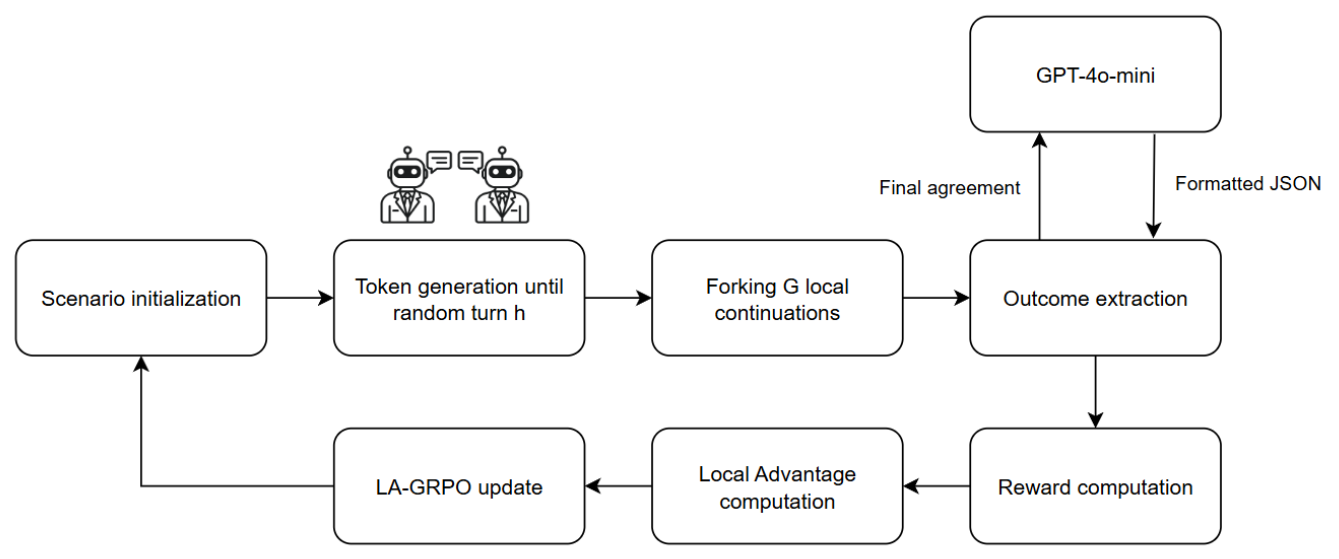
\includegraphics[width=\textwidth]{images/overview-approach.png}
    \caption{Own illustration to show the overview of the learning process.}
    \label{fig:overview}
\end{figure}

Each training iteration follows the following steps:

\begin{enumerate}
     \item \textbf{Scenario initialization}
     \newline
     Two symmetric instances of the same model (Qwen3-14B-Instruct with LoRA adapters) negotiate in natural language. The roles differ only in private payoff tables describing their preferences over issues.
     \item \textbf{Token generation until random turn $h$}
     \newline
     The dialogue proceeds token-by-token until a random negotiation turn $h$ is reached. Sampling different turns allows the algorithm to attribute downstream outcome differences to a single utterance and to spread learning evenly across the dialogue horizon.
     \item \textbf{Forking $G$ local continuations}
     \newline
     At turn $h$, the model forks $G$ continuations from the identical prefix---generating $G$ alternative offers or responses---and then completes each dialogue to termination (either agreement or no-deal). These local rollouts differ only in what $\pi_0$ says at turn $h$.
     \item \textbf{Outcome extraction}
     \newline
     Each completed dialogue is parsed by an evaluator model (GPT-4o-mini) that extracts the final agreement and detects whether a valid deal was reached. The evaluator model receives the final agreement as a string and returns a formatted JSON that allows for reward calculations.
     \item \textbf{Reward computation}
     \newline
     For each continuation, the final agreement is mapped to numeric utilities $U_A$, $U_B$ using the private payoff tables. The cooperative scalar reward combines individual and collective performance.
     \item \textbf{Computing local group-relative advantages}
     \newline
     Across the $G$ returns derived from the same context, rewards are normalized to compute local advantages. Each advantage is assigned to all tokens of turn $h$, tracing performance differences back to that specific utterance.
     \item \textbf{LA-GRPO update}
     \newline
     The model's LoRA adapters are updated by maximizing the log-probability of the tokens in higher-advantage turns while applying a KL regularization term that constrains the policy toward a frozen reference model. Only $\pi_0$ is updated; $\pi_c$ remains fixed to ensure a stationary environment.
\end{enumerate}
After updating the model's LoRA adapters, a new scenario is initialized. Because new dialogues are generated after every update, the model is constantly learning from its own evolving behavior rather than from a static dataset.


\subsection{Cooperative Reward Design}\label{sec:cooperative_reward}

\subsubsection{From Competitive to Cooperative Reward}

In \citeauthor{franceschetti2025advantage}'s (\citeyear{franceschetti2025advantage}) original formulation, each agent's return is based purely on its individual utility derived from the final negotiated outcome. This setup corresponds to zero-sum or competitive bargaining, where one party's gain is typically the other's loss and learning is driven by self-interest.
\par
In contrast, the present work extends this reward structure to non-zero-sum (mixed-motive) negotiation. Adapting LA-GRPO to this setting requires redefining the scalar reward so that it reflects not only the agent's own payoff but also the collective efficiency and equity of the final outcome.
\par
To formalize this, three cooperative criteria commonly used in bargaining theory and multi-agent reinforcement learning are introduced:

\begin{enumerate}[label={}, leftmargin=0pt]
    \item \textbf{Self-utility ($U_A$):} The agent's own payoff from the agreed outcome. This term preserves an incentive for self-interested performance. This is what was used by \citet{franceschetti2025advantage}.
    \item \textbf{Social welfare ($U_A + U_B$):} The joint utility of both parties, representing total value creation \citep{pmlr-v162-liu22l}. Maximizing this term encourages the agent to find agreements that improve overall efficiency.
    \item \textbf{Fairness / Nash product ($U_A \times U_B$):} A measure introduced by \citet{Nash1950THEBP}, which reaches its maximum when both parties achieve high and balanced payoffs. The product drops sharply if either side receives little value, implicitly penalizing unequal or exploitative deals and promoting Pareto-efficient and equitable outcomes.
\end{enumerate}

\begin{table}[H]
\centering
\caption{Theoretical grounding of cooperative reward components.}
\label{tab:reward_components}
\begin{tabular}{lll}
\toprule
\textbf{Component} & \textbf{Social welfare function} & \textbf{Property} \\
\midrule
$\lambda_{\text{self}} \cdot U_A$ & Individual rationality & Incentive to participate \\
$\lambda_{\text{welfare}} \cdot (U_A + U_B)$ & Utilitarianism (Bentham) & Maximizes total value \\
$\lambda_{\text{fair}} \cdot U_A \cdot U_B$ & Nash bargaining (Nash, 1950) & Balanced, efficient outcomes \\
\bottomrule
\end{tabular}
\end{table}

Combining these objectives yields a single scalar cooperative reward used by LA-GRPO to update the trainable policy $\pi_0$. The environment computes both agents' utilities ($U_A$, $U_B$) from their payoff tables, but only the learning agent receives the scalarized signal:

\begin{equation}
R_{\text{coop}} = \lambda_{\text{self}} \cdot U_A + \lambda_{\text{welfare}} \cdot (U_A + U_B) + \lambda_{\text{fair}} \cdot (U_A \times U_B)
\label{eq:rcoop_raw}
\end{equation}

where $\lambda_{\text{self}}$, $\lambda_{\text{welfare}}$, $\lambda_{\text{fair}} \geq 0$ are tunable coefficients balancing self-interest, total welfare and fairness. When $\lambda_{\text{welfare}} = \lambda_{\text{fair}} = 0$, this formulation reduces to Franceschetti's original self-utility reward. Increasing these parameters gradually shifts behavior toward cooperative and Pareto-efficient negotiation.
\par
This cooperative scalarization preserves the single-agent optimization loop required by LA-GRPO while embedding social objectives grounded in bargaining theory and cooperative reinforcement learning. It therefore allows the model to learn cooperation from feedback alone, without explicit prompting or role conditioning.


\subsubsection{The Scale Mismatch Problem}

The three components in Eq.~\ref{eq:rcoop_raw} operate on different scales: $U_A \in [0,100]$, welfare $\in [0,200]$, Nash product $\in [0,10{,}000]$. With equal $\lambda$ values, the welfare or Nash term dominates purely due to scale---not intentional weighting. This is particularly problematic for GRPO, where the training signal comes from the advantage $A_i = (R_i - \mu) / \sigma$ within a group: if one component's variance dominates, only that component drives the gradient.

Additional scale issues arise across game types. A distributive game may have $\max U_A = 80$ while a compatible game has $\max U_A = 100$. Without normalization, the model receives stronger gradient signal from compatible games. Furthermore, welfare has zero variance in pure distributive games ($U_A + U_B = \text{const}$), providing no learning signal at all for approximately 31\% of the training games.


\subsubsection{Solution: Game-Normalized Ratios}

$R_{\text{coop}}$ is computed using game-normalized ratios instead of raw values:

\begin{equation}
R_{\text{coop}} = \lambda_{\text{self}} \cdot \frac{U_A}{\max U_A} + \lambda_{\text{welfare}} \cdot \frac{U_A + U_B}{\max W} + \lambda_{\text{fair}} \cdot \frac{U_A \cdot U_B}{\max N}
\label{eq:rcoop_normalized}
\end{equation}

Each component is now in $[0, 1]$ regardless of game type. The function \texttt{compute\_max\_metrics()} brute-forces the per-game maximum of each component across all $\leq 121$ possible outcome combinations for two-issue games. This normalization ensures that:
\begin{enumerate}
    \item $\lambda$ values are directly interpretable as relative importance weights.
    \item Compatible and distributive games contribute equally to the gradient.
    \item No component dominates by accident.
\end{enumerate}


\subsection{Calculating Local Advantage}\label{sec:la_grpo}

Having defined the cooperative reward $R_{\text{coop}}$, the local advantage signal used by LA-GRPO to assign credit and update the policy can now be computed.
\par
To isolate the learning signal for a particular dialogue turn, this work follows \citeauthor{franceschetti2025advantage}'s (\citeyear{franceschetti2025advantage}) Local Advantage Group Relative Policy Optimization procedure. A turn $h$ is sampled from a geometric distribution $h \sim \mathrm{Geom}(0.3)$, bounded by $\max\_rounds - 1$. Rounds $0 \ldots h-1$ are played once as a shared prefix, identical across all $G$ generations. From round $h$ onward, $G$ independent continuations are generated.

The idea is to sample several continuations from the same dialogue context and measure how each continuation's final reward compares to the group's weighted average reward:

\begin{equation}
    \hat{A}_h^i = 
    \frac{R_{\text{coop}}(s_{N+1}^i) - \mathrm{mean}(\mathbf{R}_{\text{coop}}(s_{N+1}^i))}
         {\mathrm{std}(\mathbf{R}_{\text{coop}}(s_{N+1}^i))},
    \qquad i = 1, \ldots, G.
\end{equation}

This relative difference---rather than the raw return---becomes the advantage estimate for that turn. An \texttt{assistant\_mask} ensures that only agent tokens (not opponent tokens) contribute to the loss. This mask is constructed during tokenization: tokens from the agent's turns receive mask value 1, opponent turns receive 0.


\subsection{Policy Update with LoRA Adapters}

After computing the local advantage $\hat{A}_h^i$ for each sampled continuation, the trainable parameters of the negotiation model are updated through a gradient-ascent step that increases the likelihood of higher-advantage utterances. The update process follows the same optimization principle introduced by \citet{franceschetti2025advantage}, but uses the local advantage based on $R_{\text{coop}}$ instead of the purely self-interested payoff.

Formally, the objective for the update step is defined as:
\begin{equation}
L = - \frac{1}{G} \sum_{i=1}^{G}\sum_{t=1}^{T_i}
    \frac{\pi_{\theta}(a_{h,t}^i|s_{h,t}^i)}{\pi_{\text{old}}(a_{h,t}^i|s_{h,t}^i)}
    \hat{A}_h^i
    + \beta \, D_{\mathrm{KL}}\!\left[\pi_{\theta}(a_{h,t}^i|s_{h,t}^i) \,\|\, \pi_{\mathrm{ref}}(a_{h,t}^i|s_{h,t}^i)\right]
\end{equation}

The first term maximizes the log-probability of tokens belonging to high-advantage turns, therefore reinforcing actions that produced cooperative and Pareto-efficient outcomes. The second term applies \textit{KL-regularization} to constrain the updated policy toward the frozen reference model $\pi_{\mathrm{ref}}$, preventing language drift or reward hacking.

Only a low-rank subset of parameters---the \textbf{LoRA adapters}---is trainable \citep{hu2021loralowrankadaptationlarge}. This modular fine-tuning strategy allows efficient weight updates on limited hardware while preserving the base model's general linguistic competence.

\paragraph{Choice of Model.}
\citet{franceschetti2025advantage} used LLaMA~3.1~8B as the base model for both negotiation agents. In this work, \textbf{Qwen3-14B-Instruct} is used instead for three reasons.

First, cooperative negotiation places higher demands on reasoning and pragmatic language use than competitive bargaining: the agent must simultaneously track its own payoff, infer the opponent's preferences, and identify mutually beneficial trade-offs. A larger model (14B vs.\ 8B parameters) provides greater capacity for this multi-objective reasoning.

Second, Qwen3 is a more recent model family with stronger instruction-following capabilities. This proved critical in early experiments: LLaMA~3.1~8B frequently violated the negotiation protocol by leaking private payoff table values to the opponent (e.g., stating ``R\&D budget of \$8M gives me a payoff of 40'') and by inventing issues that did not exist in the scenario configuration. Both behaviors are particularly damaging for cooperative training, where the reward signal depends on the agent negotiating \textit{within} the defined game structure. A model that fabricates issues or reveals its payoff function undermines the integrity of the training loop, as the evaluator cannot correctly extract outcomes from such dialogues. Qwen3-14B exhibited these problems far less frequently, and the remaining instances diminished further as training progressed.

Third, with 4-bit quantization (BitsAndBytes nf4), Qwen3-14B fits comfortably on a single RTX~5090 (32\,GB) or A100 (80\,GB), making it practical for the single-GPU training pipeline used in this work. The LoRA configuration ($r=8$, $\alpha=16$, dropout$=0.1$) is kept identical to Franceschetti's to isolate the effect of the model change from other variables.

The specific model and LoRA configuration are:

\begin{itemize}
    \item \textbf{Base model:} Qwen3-14B-Instruct, loaded in 4-bit quantization (BitsAndBytes nf4, double quant, bf16 compute dtype)
    \item \textbf{LoRA:} $r=8$, $\alpha=16$, dropout $= 0.1$, applied to all linear modules
    \item \textbf{Reference model:} Same model with LoRA disabled (no additional VRAM required)
    \item \textbf{Opponent:} Frozen local model with LoRA disabled
    \item \textbf{Loss type:} GRPO (explicitly set; TRL 0.29+ defaults to DAPO)
\end{itemize}

After each policy update, the LoRA weights are merged with the frozen base model to form a new active policy $\pi_{\theta}^{\text{new}}$. The negotiation loop then restarts with fresh self-play dialogues generated from this updated policy, keeping the procedure \textit{fully on-policy}. Because dialogues and rewards are regenerated after every iteration, the model continuously learns from its own evolving negotiation behaviour.


\subsection{Expected Effects and Hypotheses}\label{sec:hypotheses}

Based on the theoretical framework and reward design, the following hypotheses are formulated:

\begin{enumerate}[label=\textbf{H\arabic*:}]
    \item Fair-only ($\lambda_{\text{fair}}=1.0$) achieves higher agreement rate than self-only ($\lambda_{\text{self}}=1.0$), because the Nash product rewards balanced outcomes where both parties benefit. Under self-only, the agent can obtain high reward by squeezing the opponent (e.g., $U_A=80, U_B=10$), but such lopsided offers are more likely to be rejected. Under Nash product, only mutually beneficial agreements yield high reward ($50 \times 50 = 2500 \gg 80 \times 10 = 800$), so the agent learns to make offers the opponent is willing to accept.
    \item Self-only extracts more $U_A$ but at the expense of $U_B$ and overall efficiency.
    \item All-equal ($\lambda_{\text{self}} = \lambda_{\text{welfare}} = \lambda_{\text{fair}} = 1.0$) underperforms because the welfare term provides no signal in distributive games.
    \item Cooperative training generalizes to unseen games (e.g., Trust Game) through transfer of cooperative disposition.
\end{enumerate}


% ============================================================
% 4. EXPERIMENTAL SETUP
% ============================================================
\newpage
\section{Experimental Setup}
\label{sec:experimental_setup}

This chapter describes how experiments are designed to test the cooperative LA-GRPO framework. It covers the LAMEN negotiation environment, issue sampling, evaluation pipeline, and ethical considerations.

\subsection{Negotiation Environment (LAMEN)}

The negotiation tasks are defined using the LAMEN framework \citep{davidson2024evaluatinglanguagemodelagency}, which provides standardized, YAML-based multi-issue bargaining games. Each scenario specifies roles, issues, and payoff tables that determine agents' private utilities. LAMEN's modular structure allows easy configuration of integrative and mixed-motive games, essential for testing cooperation. Scenario definitions are loaded dynamically using the Hydra configuration system, which supports hierarchical experiment management and parameter overrides. The turn-taking protocol and evaluation prompts follow Franceschetti's original implementation and LAMEN's reference design, ensuring full comparability. The framework's modular design covers four configuration layers:

\begin{enumerate}[label={}, leftmargin=0pt]
    \item \textbf{Games:} Each game file defines the scenario context and the set of issues and their possible outcomes.
    \item \textbf{Issues:} Every issue is accompanied by private payoff values for each agent. Every payoff value also contains a corresponding label (e.g.\ value: 10, label: \$10). This allows the use and combination of different issues for various types of games.
    \item \textbf{Agent roles:} Agent roles define each of the two LLMs with name, gender, profession, age and personality type. This file provides an internal and external description. The internal description is only accessible to the agent itself, while the external description can also be seen by the opposing agent.
    \item \textbf{Rules:} The rules are based on the Rio Copa game \citep{bontempo2008riocopa}. It defines prompts such as to never make offers that are not part of the possible values in the payoff table.
\end{enumerate}

The turn-taking protocol follows an alternating-offer design with 5 rounds per agent ($N=5$), and start order is alternated across episodes to counteract the anchoring effect \citep{tversky1974judgment}. Outcome extraction is performed by GPT-4o-mini, which parses negotiation transcripts and returns structured JSON with agreed values per issue. \citet{franceschetti2025advantage} verified 98\% extraction accuracy across 500 samples.


\subsection{Game and Issue Design}

Depending on how the payoff values align between the two agents, LAMEN categorizes games into four archetypes:

\begin{figure}[H]
    \centering
    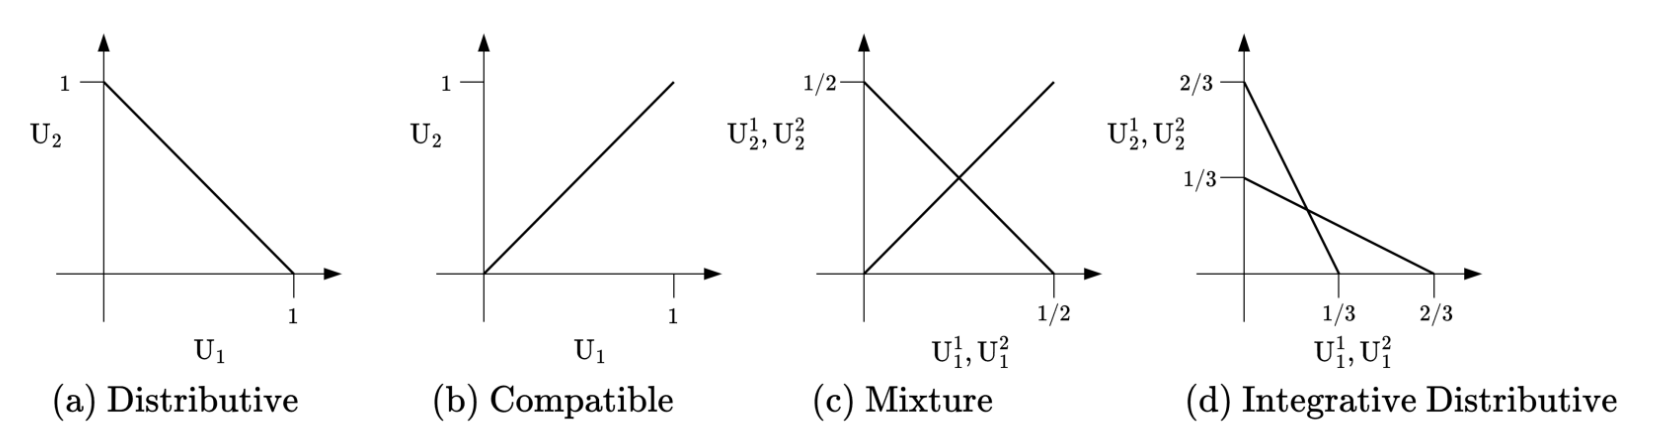
\includegraphics[width=\textwidth]{images/lamen-archetypes.png}
    \caption{Four archetypes of negotiation games \citep{davidson2024evaluatinglanguagemodelagency}}
    \label{fig:archetypes}
\end{figure}

\begin{enumerate}[label={}, leftmargin=0pt]
    \item \textbf{Distributive:} All issues are purely competitive (zero-sum)---one agent's gain is the other's loss. For a single-issue distributive game, the agents' interests directly oppose each other \citep{davidson2024evaluatinglanguagemodelagency}. A typical example is splitting a fixed resource: if two friends split a pizza, each extra slice for Alice is a slice Bob cannot have.
    \item \textbf{Compatible:} All issues are fully aligned---both agents prefer the same outcomes. In a compatible single-issue game, there is no conflict of interest \citep{davidson2024evaluatinglanguagemodelagency}. For instance, if both parties benefit from adding extra cheese on a pizza, deciding the cheese amount is a compatible issue.
    \item \textbf{Mixture:} Games that include multiple issues with a mix of distributive and compatible \citep{davidson2024evaluatinglanguagemodelagency}. For example, a two-issue game might have one issue being distributive (e.g.\ splitting slices of pizza) and another issue compatible (e.g.\ both want more cheese).
    \item \textbf{Integrative-Distributive:} Multi-issue games where all issues are in themselves contested (distributive), but the agents attach different importance weights to each issue. This asymmetric preference structure creates opportunities for integrative trade-offs \citep{davidson2024evaluatinglanguagemodelagency}. Each agent values the issues differently, so they can cooperate by conceding on less-important issues in exchange for gains on more-important issues.
\end{enumerate}

This work focuses on \textit{mixed-motive} games---games in which agents face both competitive and cooperative incentives simultaneously. In game theory, mixed-motive describes any setting where players' interests are neither fully opposed (as in pure distributive games) nor fully aligned (as in pure compatible games), but contain elements of both. In the LAMEN framework, the \textit{Mixture} and \textit{Integrative-Distributive} archetypes are mixed-motive: both require the agent to navigate competitive dynamics on some issues while finding mutually beneficial trade-offs on others. The training set also includes a small proportion of purely compatible games, where both agents' interests are fully aligned.

\paragraph{Extended Game Set.} This work extends Franceschetti's game set from 3 scenarios, 10 issues, and 23 game combinations to \textbf{5 scenarios, 19 issues, and 47 game configurations} (19 single-issue and 28 two-issue, with one conflicting combination excluded):

\begin{table}[H]
\centering
\caption{Negotiation scenarios and their issues.}
\label{tab:scenarios}
\begin{tabular}{lp{5.5cm}c}
\toprule
\textbf{Scenario} & \textbf{Issues} & \textbf{Source} \\
\midrule
Generic Rental Agreement & 4 issues \newline \textit{(rent, duration, deposit, maintenance)} & Franceschetti \\
\addlinespace
Generic Loan Agreement & 3 issues \newline \textit{(rate, term, collateral)} & Franceschetti \\
\addlinespace
Generic Merger & 3 issues \newline \textit{(valuation, retention, governance)} & Franceschetti \\
\addlinespace
Joint Venture & 4 issues \newline \textit{(R\&D budget, revenue split, data sharing, authority)} & New \\
\addlinespace
Employment Contract & 5 issues \newline \textit{(salary, remote work, training, equity, scope)} & New \\
\bottomrule
\end{tabular}
\end{table}

For multi-issue training, two issues $(i_1, i_2)$ are drawn at random from the selected scenario's issue pool. Each issue has its own payoff table and importance weighting vector $(\omega_{A,1}, \omega_{A,2})$ sampled from $\{(0.9, 0.1), (0.5, 0.5), (0.1, 0.9)\}$. This variation forces the agent to identify which issue carries higher value in each game and to negotiate trade-offs accordingly. One issue may be distributive while the other is compatible, resulting in a mixed-motive negotiation that combines competitive and cooperative objectives within a single dialogue.

The resulting game combinations fall into three archetypes:

\begin{table}[H]
\centering
\caption{Distribution of game archetypes in the training set.}
\label{tab:archetypes_dist}
\begin{tabular}{llc}
\toprule
\textbf{Archetype} & \textbf{Description} & \textbf{Share} \\
\midrule
Compatible & Both agents prefer the same outcome & 7\% \\
Mixture & Mix of distributive and compatible issues & 69\% \\
Integrative-Distributive & All contested, but different importance weights & 24\% \\
\bottomrule
\end{tabular}
\end{table}

This distribution is a deterministic consequence of the issue pool composition: each issue has a fixed payoff structure (distributive or compatible), and the archetype of a two-issue game is fully determined by the types of its constituent issues. Issues were designed for ecological validity rather than artificial balance---in a real employment contract, salary is inherently distributive while training budget is naturally compatible. The resulting dominance of mixture games is desirable for this work: these mixed-motive settings require agents to balance competitive and cooperative behavior, which is the core challenge this thesis addresses. \citet{davidson2024evaluatinglanguagemodelagency} similarly found that cooperative bargaining games proved to be the most challenging for LLMs, further motivating their prominence in the training set.

Two game-type configurations are supported:
\begin{itemize}
    \item \texttt{multi-game}: All 5 scenarios (used for the main experiments)
    \item \texttt{out-of-domain}: Rio Copa scenario (evaluation only)
\end{itemize}

During the initialization of a scenario, a random game with random issues from a pre-defined set is chosen. This prevents overfitting to one specific case as it includes different kinds of scenarios with unique payoff tables.


\subsection{Agent Roles and Initialization}

Two symmetric instances of the same model are assigned roles with distinct names, professions, ages, and personality types. Each agent has access only to its own private payoff table. The system prompt explicitly forbids revealing payoff information to the opponent.

At the start of each episode, the initial prompt $s_0$ is constructed by inserting the scenario description, role information, and payoff tables of the sampled issues. The model then conducts a full negotiation consisting of five rounds per agent ($N=5$), alternating roles across episodes to avoid first-mover bias. During LA-GRPO training, the turn $h$ at which the dialogue diverges into multiple continuations is drawn from a geometric distribution $h \sim \mathrm{Geom}(0.3)$, prioritizing early turns where strategic anchors typically emerge \citep{franceschetti2025advantage}.

To provide an intuitive illustration of the negotiation setup, Appendix~\ref{app:example_dialogue} presents a simplified and hypothetical example of a mixed-motive self-play dialogue.


\subsection{Training Configurations ($\lambda$ Ablation)}

Five $\lambda$ configurations are trained with GRPO to explore the effect of each reward component. Three of these---self-only, fair-only, and all-equal---are retrained with LA-GRPO. The remaining two (welfare-only and self-fair-equal) are omitted from LA-GRPO training to reduce compute costs, since LA-GRPO requires more steps per run.

\begin{table}[H]
\centering
\caption{$\lambda$ configurations and training methods. LA-GRPO trains for more steps but uses fewer tokens per step (shared dialogue prefix generated once per group).}
\label{tab:lambda_configs}
\begin{tabular}{lccclcc}
\toprule
\textbf{Run} & $\lambda_{\text{s}}$ & $\lambda_{\text{w}}$ & $\lambda_{\text{f}}$ & \textbf{Method} & \textbf{Steps} \\
\midrule
Base Model & --- & --- & --- & --- & 0 \\
Self-Only & 1.0 & 0.0 & 0.0 & GRPO + LA-GRPO & 560 / 2000 \\
Fair-Only & 0.0 & 0.0 & 1.0 & GRPO + LA-GRPO & 560 / 1340 \\
Welfare-Only & 0.0 & 1.0 & 0.0 & GRPO only & 560 \\
All-Equal & 1.0 & 1.0 & 1.0 & GRPO + LA-GRPO & 620 / 2000 \\
Self-Fair-Equal & 1.0 & 0.0 & 1.0 & GRPO only & 820 \\
\bottomrule
\end{tabular}
\end{table}

The first three configurations isolate the effect of each individual reward component. All-equal combines all three terms with equal weight. Self-fair-equal tests whether the welfare component can be dropped without loss of performance, giving equal weight to self-interest and fairness only.

For each training step, $G = 8$ independent dialogue continuations are generated per prompt. Training progress is logged via Weights \& Biases, with the game-normalized \texttt{ratio\_rcoop} serving as the primary training metric. All model weights, configuration files, and generated dialogues are version-controlled using GitHub to ensure reproducibility.

Table~\ref{tab:hyperparams} lists the full training hyperparameters, which are shared across all $\lambda$ configurations. The optimizer is AdamW (fused variant) with a learning rate of $5 \times 10^{-5}$ and a constant-with-warmup schedule (10 warmup steps). The KL penalty coefficient $\beta = 0.08$ constrains the policy from diverging too far from the frozen reference model, while the clipping threshold $\epsilon = 0.2$ bounds the importance ratio $\pi_\theta / \pi_{\text{old}}$ to $[1 - \epsilon, 1 + \epsilon]$ in the GRPO loss. In practice, clipping never triggered during training (clip ratio remained at 0 across all runs), indicating that the LoRA-based updates are sufficiently conservative. Generation temperature is set to $1.0$ to encourage diverse dialogue continuations across the $G = 8$ samples. Gradient checkpointing is enabled to reduce memory usage at the cost of slightly longer step times.

\begin{table}[H]
\centering
\caption{Training hyperparameters (shared across all $\lambda$ configurations).}
\label{tab:hyperparams}
\renewcommand{\arraystretch}{1.15}
\begin{tabular}{ll}
\toprule
\textbf{Parameter} & \textbf{Value} \\
\midrule
Optimizer & AdamW (fused), $\beta_1 = 0.9$, $\beta_2 = 0.999$, $\epsilon = 10^{-8}$ \\
Learning rate & $5 \times 10^{-5}$ \\
LR schedule & Constant with warmup (10 steps) \\
Weight decay & 0 \\
Batch size & 8 per device, gradient accumulation $= 1$ \\
KL coefficient ($\beta$) & 0.08 \\
Clipping threshold ($\epsilon$) & 0.2 \\
Max grad norm & 1.0 \\
Generation temperature & 1.0 \\
Generations per prompt ($G$) & 8 \\
Max tokens per turn & 200 \\
Precision & bf16 \\
Gradient checkpointing & Enabled \\
Eval / save interval & Every 20 steps \\
Seed & 42 \\
\bottomrule
\end{tabular}
\end{table}


\subsection{Technical Setup}\label{sec:technical}

\paragraph{Infrastructure and GPU Migration.}
\citet{franceschetti2025advantage}'s original training pipeline required four GPUs: two NVIDIA A100s running vLLM inference servers (one for the policy model $\pi_\theta$ and one for the frozen opponent $\pi_c$) and two additional A100s for gradient computation. This setup enabled batched dialogue generation via vLLM's paged attention mechanism \citep{kwon2023efficientmemorymanagementlarge}, significantly accelerating the sampling of multiple continuations per training step.

Due to cost constraints, this work rewrites the training pipeline to operate on a \textbf{single GPU}. Training is performed on a rented NVIDIA A100 (80\,GB), which provides sufficient memory for the model, LoRA adapters, optimizer states, and the long KV caches produced by multi-turn dialogues. Evaluation and smaller experiments are run on a rented NVIDIA RTX~5090 (32\,GB), which is adequate for inference but lacks the memory headroom required for stable gradient accumulation during training. Both the policy model and the frozen opponent run on the same device, with LoRA adapters enabled or disabled to switch between the two roles. This eliminates the need for inter-GPU communication and multi-server orchestration, substantially reducing infrastructure complexity and cost. The trade-off is the loss of vLLM: since a single GPU cannot simultaneously host a vLLM inference server and perform gradient updates, dialogue generation falls back to sequential \texttt{model.generate()} calls. Each training step requires approximately 80 forward passes ($G = 8$ continuations $\times$ up to 10 dialogue turns), resulting in step times of 100--150 seconds. While a vLLM colocate mode was planned to recover batched generation on a single GPU, it was not implemented within the scope of this thesis due to a technical incompatibility: TRL's vLLM colocate mode requires vLLM to manage model loading, which conflicts with the BitsAndBytes 4-bit quantization pipeline used for training---the two model loading approaches cannot coexist on a single GPU.

\paragraph{Model and Quantization.}
To fit Qwen3-14B on a single GPU, BitsAndBytes 4-bit quantization is applied (nf4 data type, double quantization, bf16 compute dtype). This reduces the model's memory footprint from $\sim$28\,GB (fp16) to $\sim$9\,GB, leaving sufficient headroom for LoRA adapters, optimizer states, and KV cache during generation.


\subsection{Evaluation Pipeline}

\subsubsection{Training Monitoring}

Training progress is tracked via Weights \& Biases (WandB). At each training step, the following metrics are logged from the negotiation that was just played:

\begin{itemize}
    \item \textbf{Reward metrics:} The composite cooperative reward $R_{\text{coop}}$ and its game-normalized ratio \texttt{ratio\_rcoop}, as well as the individual components \texttt{ratio\_self}, \texttt{ratio\_welfare}, and \texttt{ratio\_nash} (each in $[0, 1]$).
    \item \textbf{Agreement rate:} The fraction of negotiations that result in a deal.
    \item \textbf{Agreed-only metrics:} The same reward ratios computed exclusively over successful negotiations, separating deal quality from deal quantity.
    \item \textbf{Training diagnostics:} KL divergence between the current policy and the reference model, reward standard deviation across the $G$ continuations, training tokens consumed, and step time.
\end{itemize}

These metrics serve as an early signal for training dynamics (e.g., detecting reward collapse or KL divergence spikes) but are noisy due to the small sample size per step. All quantitative results reported in Chapter~\ref{sec:results} are therefore based on the post-training evaluation described below.

\subsubsection{Post-Training Evaluation}

Each trained model is evaluated by playing selfplay negotiations against the frozen base model opponent (LoRA disabled). The evaluation dataset consists of \textbf{14 game configurations} drawn from the training set, covering all 7 archetypes. Each configuration is played in both starting roles (agent starts first vs.\ opponent starts first), yielding 28 games per repetition. With \textbf{20 repetitions} per model, this produces a total of \textbf{560 evaluated negotiations} per model. Each repetition uses a different random seed (base seed $= 42$, incremented per repetition) to ensure variation in generation while maintaining reproducibility.

Generation uses temperature $= 1.0$ with a maximum of 200 tokens per turn and 5 negotiation rounds per agent. The same generation parameters are applied to all models to ensure a fair comparison.

A negotiation is classified as \textit{agreed} if either agent receives a positive payoff ($U_A > 0$ or $U_B > 0$).

Since negotiation payoffs are not normally distributed (failed negotiations produce zeros, creating a bimodal distribution), non-parametric statistical tests are used throughout:

\begin{itemize}
    \item \textbf{Mann-Whitney U test:} For pairwise comparison of continuous metrics ($U_A$, ratio Nash, ratio welfare) between two models. Two-sided, with significance levels $^* p < 0.05$, $^{**} p < 0.01$, $^{***} p < 0.001$.
    \item \textbf{Chi-squared test:} For comparing binary agreement rates between models, using $2 \times 2$ contingency tables.
    \item \textbf{Bootstrap confidence intervals:} 95\% CIs computed via non-parametric bootstrap with 10{,}000 resamples.
\end{itemize}

\subsubsection{Out-of-Domain: Trust Game}

To test generalization, the Trust Game is used as an out-of-domain evaluation---a 2-turn game-theoretic setting the model was never trained on:
\begin{itemize}
    \item \textbf{Rules:} Investor sends $x \in [0, 10]$ points (tripled to $3x$). Trustee returns $y \in [0, 3x]$.
    \item \textbf{Nash equilibrium:} send $= 0$ (selfish rational). \textbf{Pareto optimum:} send $= 10$, return $= 15$.
    \item \textbf{Conditions:} \texttt{vs\_base} (trained model vs.\ frozen base) and \texttt{vs\_self} (selfplay).
    \item 50 games per condition for GRPO, 300 for LA-GRPO, temperature $= 1.0$, seed $= 42$.
\end{itemize}

\subsubsection{Language and Generalization Tests}

To verify that alignment on negotiation tasks does not harm general capabilities, the GRPO and LA-GRPO all-equal models are re-evaluated on three standard benchmarks using the Language Model Evaluation Harness \citep{eval-harness} with a vLLM backend:

\begin{itemize}
    \item \textbf{MMLU-Pro} \citep{wang2024mmluprorobustchallengingmultitask}: 5-shot multiple-choice evaluation across 14 academic subjects (12{,}000+ questions with 10 answer options). Tests factual knowledge and reasoning.
    \item \textbf{IFEval} \citep{zhou2023instructionfollowingevaluationlargelanguage}: 541 prompts with 1{,}500+ atomic constraints testing fine-grained instruction following (formatting, structural constraints, stylistic directives). Reported as prompt-level strict accuracy.
    \item \textbf{GSM8K}: 8.5K grade-school math word problems requiring multi-step arithmetic reasoning. Reported as strict-match accuracy.
\end{itemize}



% ============================================================
% 5. RESULTS AND DISCUSSION
% ============================================================
\newpage
\section{Results and Discussion}
\label{sec:results}

\subsection{Training Dynamics and Convergence}

This section describes how the models behave during training. Two sets of training curves are shown---GRPO (Figures~\ref{fig:training_performance} and~\ref{fig:training_quality}) and LA-GRPO (Figures~\ref{fig:lagrpo_training_performance} and~\ref{fig:lagrpo_training_quality})---and discussed in turn. All curves are smoothed with a centered running average (window $= 100$ data points).

\subsubsection{GRPO Training Dynamics}

GRPO runs were all capped at 600 steps to keep compute costs manageable. Five $\lambda$ configurations were trained.

\begin{figure}[H]
    \centering
    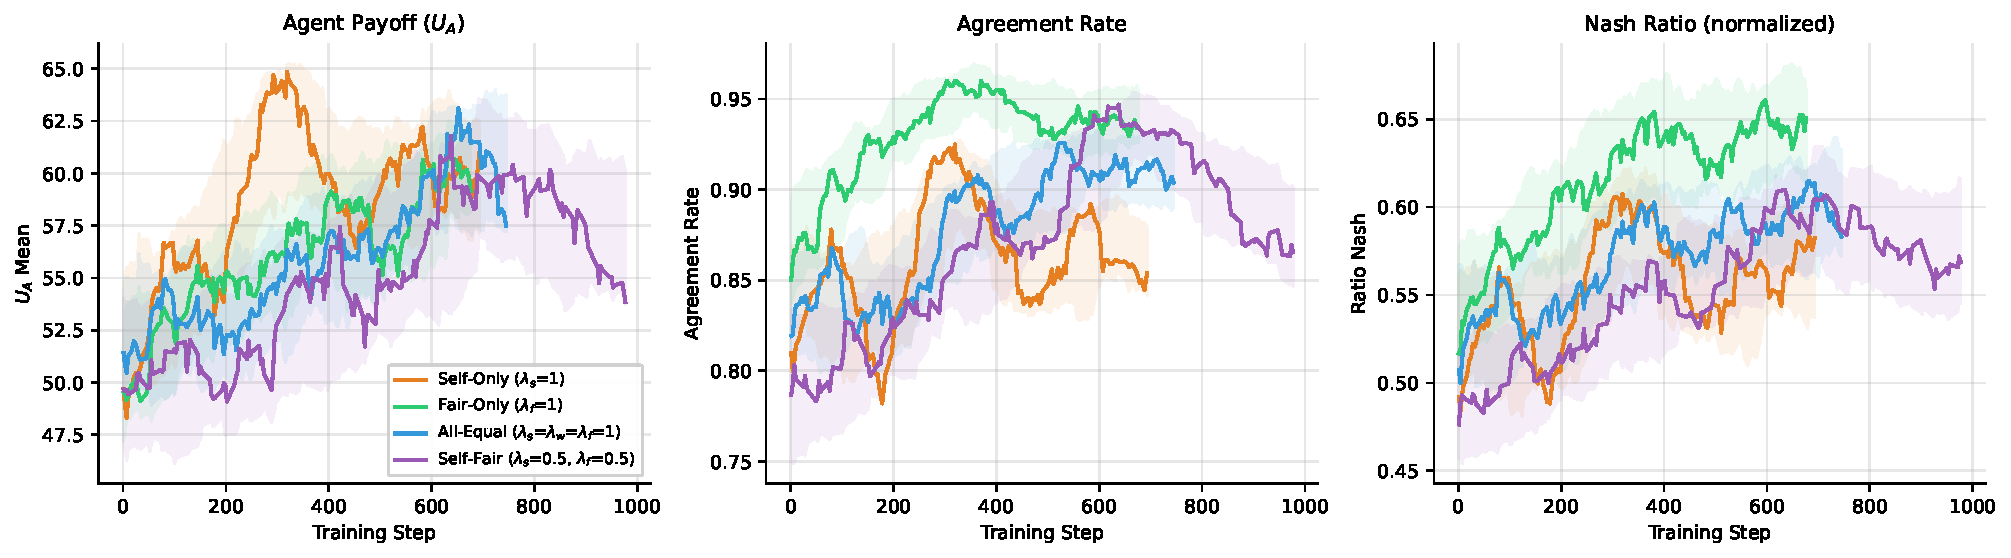
\includegraphics[width=\textwidth]{images/training_curves_performance.pdf}
    \caption{GRPO negotiation performance during training across five $\lambda$ configurations. All curves are smoothed with a centered running average (window $= 100$ data points). Shaded regions indicate variance. Top left: mean agent payoff $U_A$. Top right: agreement rate. Bottom left: normalized Nash ratio. Bottom right: normalized welfare ratio. Fair-only and all-equal show the strongest cooperative improvements, while self-only improves $U_A$ but not cooperative metrics. Welfare-only performs similarly to self-only on most metrics.}
    \label{fig:training_performance}
\end{figure}

\begin{figure}[H]
    \centering
    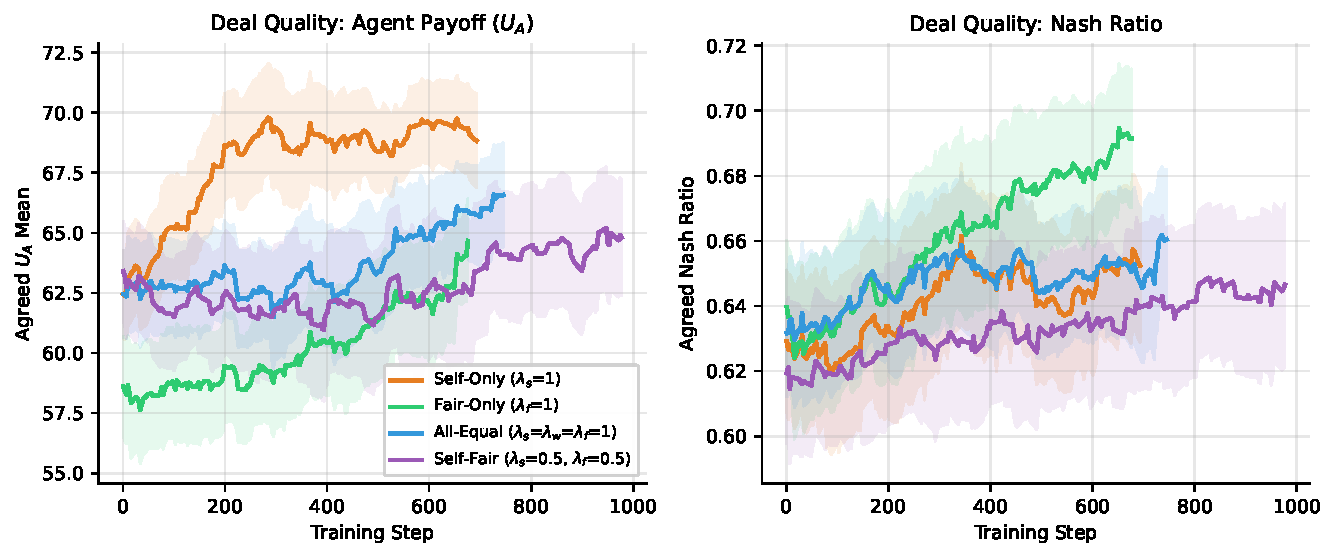
\includegraphics[width=\textwidth]{images/training_curves_quality.pdf}
    \caption{GRPO deal quality during training, computed only over successful negotiations. Left: agreed $U_A$ (excluding failed negotiations). Right: agreed Nash ratio. Self-only achieves the highest individual payoff on agreed deals, while fair-only leads on balanced outcomes. Welfare-only shows declining Nash ratio after step $\sim$400, suggesting over-optimization toward total value at the expense of balanced deals.}
    \label{fig:training_quality}
\end{figure}

\paragraph{Reward function shapes learning.} Under GRPO self-only, agreement rate plateaus at a lower level than under fair-only or all-equal. This is consistent with H1 (Section~\ref{sec:hypotheses}): the Nash product reward incentivizes mutually acceptable offers, while pure self-interest can produce lopsided proposals that the opponent rejects.

\paragraph{Self-only fails to improve Nash product (under GRPO).} GRPO self-only's Nash ratio plateaus near the base model's level---pure self-interest provides no cooperative improvement over the untrained model. The agent extracts more for itself (higher $U_A$) but at the expense of the opponent. This pattern matches H2 (Section~\ref{sec:hypotheses}).

\paragraph{Fair-only diverges more from the base model.} The KL divergence between policy and reference model is higher for GRPO fair-only (KL $0.22$--$0.62$) than for self-only (KL $0.07$--$0.13$), indicating a stronger learning signal from the Nash product reward. While this is not yet in a concerning range, it warrants monitoring for potential instability. Reinforcement learning methods like PPO or GRPO are known to induce over-optimization or ``language drift'' when hyperparameters are mis-set \citep{pmlr-v235-jang24b, ouyang2022traininglanguagemodelsfollow}.

\subsubsection{LA-GRPO Training Dynamics}

The three LA-GRPO configurations (self-only, fair-only, all-equal) were trained for up to 2000 steps, with fair-only stopping at step $\sim$1200.

\begin{figure}[H]
    \centering
    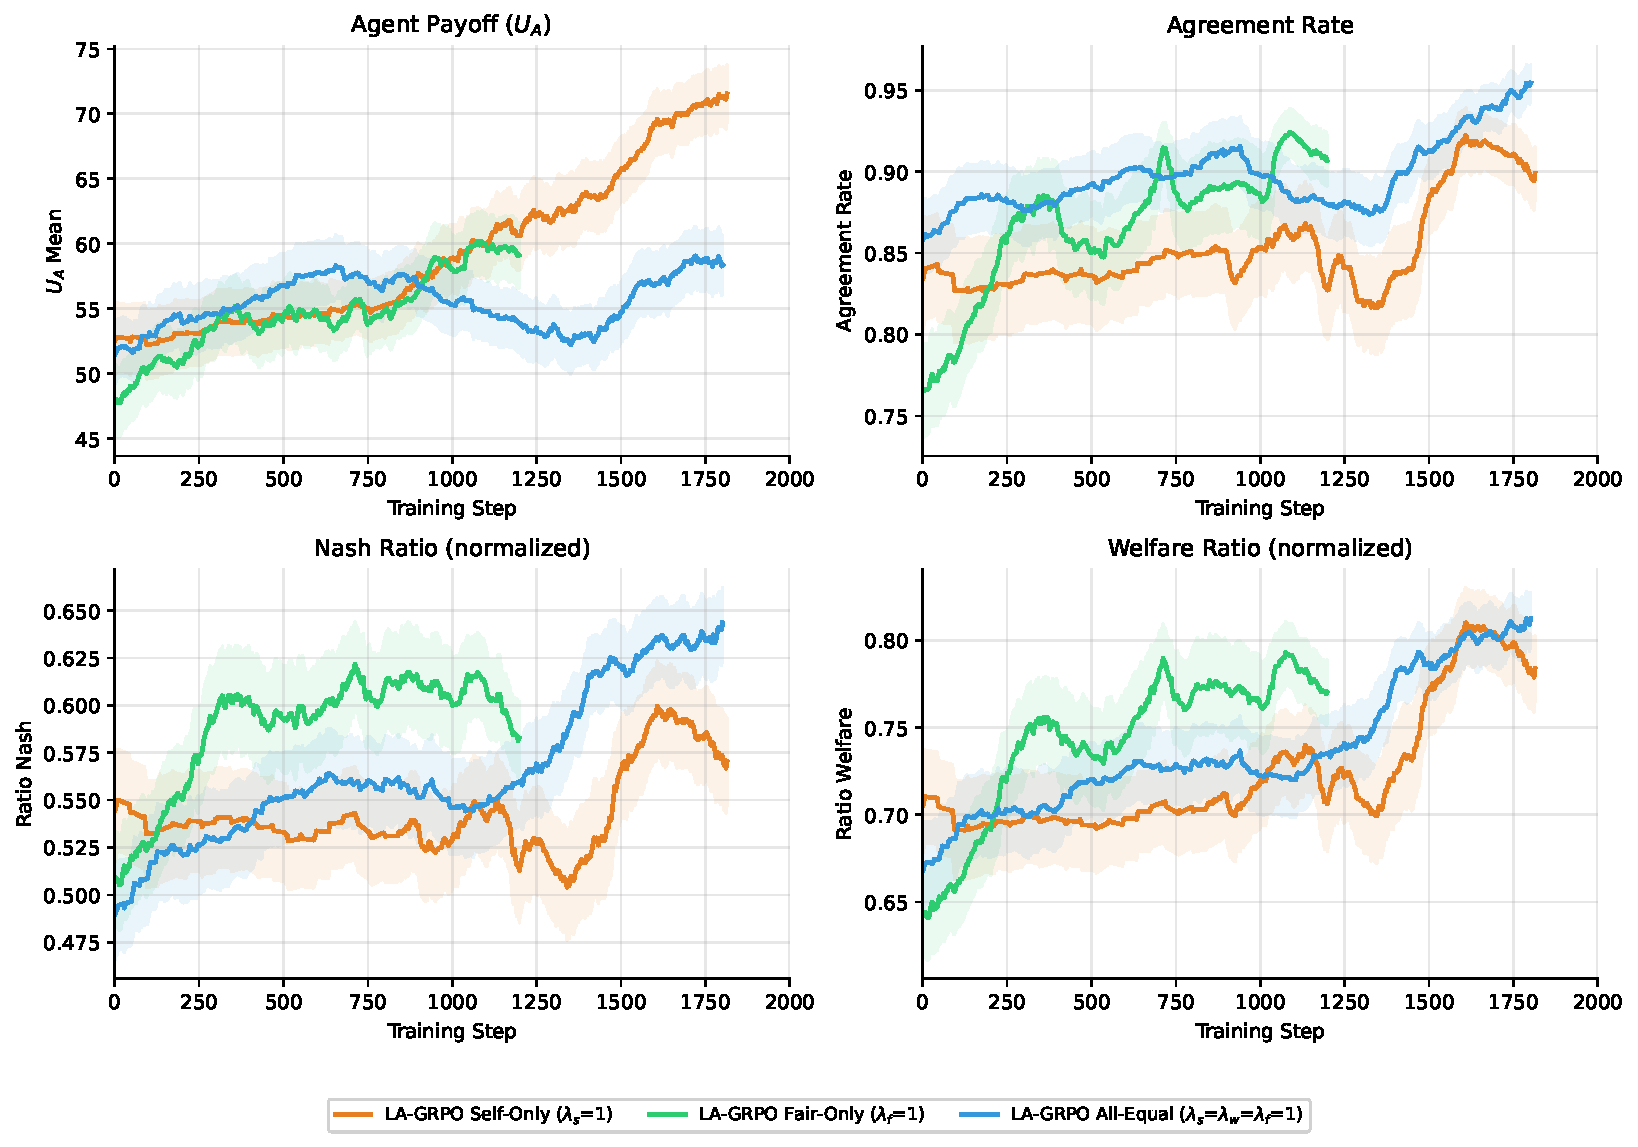
\includegraphics[width=\textwidth]{images/lagrpo_training_curves_performance.pdf}
    \caption{LA-GRPO negotiation performance during training across three $\lambda$ configurations (up to 2000 steps). Same smoothing and layout as Figure~\ref{fig:training_performance}. Self-only continues to improve over the full training range, while fair-only (whose run was terminated earlier) reaches high Nash and welfare ratios more quickly.}
    \label{fig:lagrpo_training_performance}
\end{figure}

\begin{figure}[H]
    \centering
    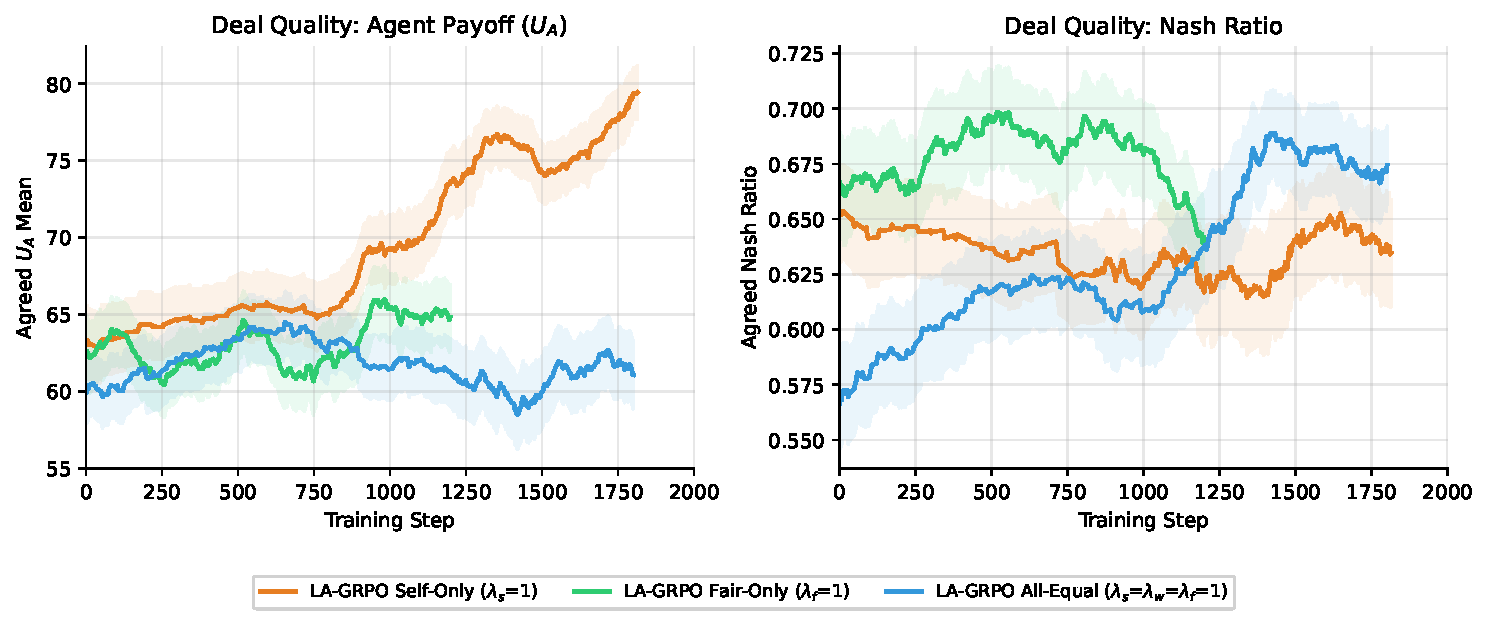
\includegraphics[width=\textwidth]{images/lagrpo_training_curves_quality.pdf}
    \caption{LA-GRPO deal quality during training, computed only over successful negotiations. Left: agreed $U_A$. Right: agreed Nash ratio. Self-only's agreed $U_A$ rises sharply, indicating increasingly aggressive value extraction, while its agreed Nash ratio remains flat. Fair-only reaches the highest agreed Nash ratio ($\sim 0.70$) around step 1000--1400 before slowly declining, suggesting the onset of over-optimization; the evaluated checkpoint (1340) was selected near this peak.}
    \label{fig:lagrpo_training_quality}
\end{figure}

\paragraph{Self-only continues to improve.} Unlike GRPO self-only, which plateaus, LA-GRPO self-only shows continued improvement in $U_A$ over the full 2000 training steps. This suggests that turn-level credit assignment extracts more learning signal from the same reward, though---as the post-training evaluation in Section~\ref{sec:grpo_vs_lagrpo} will show---most of this gain is in raw $U_A$ rather than cooperative quality.

\paragraph{Checkpoint selection matters for LA-GRPO fair-only.} Figure~\ref{fig:lagrpo_training_quality} shows that the agreed Nash ratio for LA-GRPO fair-only rises to a peak of approximately $0.70$ around step 1000--1400, then gradually declines toward $0.66$ by step 2000. This pattern is consistent with reward hacking or mild over-optimization: after the model has converged on a cooperative strategy, continued training begins to degrade the quality of individual deals. Based on this observation, checkpoint 1340 (near the peak) was selected for the post-training evaluation of LA-GRPO fair-only, rather than the final checkpoint. For the other LA-GRPO configurations, which did not exhibit a clear decline, the last checkpoint (step 2000) was used.

The following sections (5.2--5.4) present the formal post-training evaluation with statistical tests, per-archetype breakdowns, and the direct GRPO vs.\ LA-GRPO comparison.


\subsection{GRPO Negotiation Performance}

Table~\ref{tab:eval_results} presents the main evaluation results across all GRPO model configurations. Each model was evaluated on 560 games (14 configurations $\times$ 2 starting roles $\times$ 20 repetitions), covering all 7 archetypes with a balanced representation. All games are played in selfplay against the frozen base model opponent, with GPT-4o-mini as outcome judge, temperature $= 1.0$, and seed $= 42$.

\begin{table}[H]
\centering
\caption{GRPO negotiation evaluation results (20 repetitions, 560 games per model). Bold indicates best per column. 95\% bootstrap confidence intervals in brackets.}
\label{tab:eval_results}
\renewcommand{\arraystretch}{1.15}
\begin{tabular}{lccccc}
\toprule
\textbf{Model} & $\lambda$ \textbf{(s/w/f)} & \textbf{Agreement} & $\mathbf{U_A}$ \textbf{mean} & \textbf{Ratio Welfare} & \textbf{Ratio Nash} \\
\midrule
Base Model & --- & 78.6\% & 49.9 \scriptsize{[47.2, 52.6]} & 0.702 \scriptsize{[0.671, 0.734]} & 0.585 \scriptsize{[0.556, 0.613]} \\
Self-Only & 1/0/0 & 79.8\% & 54.9 \scriptsize{[52.0, 57.7]} & 0.723 \scriptsize{[0.691, 0.753]} & 0.581 \scriptsize{[0.552, 0.610]} \\
Fair-Only & 0/0/1 & 89.6\% & 55.0 \scriptsize{[52.4, 57.6]} & 0.808 \scriptsize{[0.782, 0.833]} & 0.664 \scriptsize{[0.637, 0.689]} \\
Welfare-Only & 0/1/0 & 85.9\% & 57.5 \scriptsize{[54.8, 60.0]} & 0.778 \scriptsize{[0.751, 0.805]} & 0.641 \scriptsize{[0.615, 0.668]} \\
\textbf{All-Equal} & \textbf{1/1/1} & \textbf{92.7\%} & \textbf{60.3} \scriptsize{[58.0, 62.6]} & \textbf{0.840} \scriptsize{[0.819, 0.861]} & \textbf{0.692} \scriptsize{[0.669, 0.716]} \\
Self-Fair-Equal & 1/0/1 & 83.8\% & 57.0 \scriptsize{[54.4, 59.6]} & 0.757 \scriptsize{[0.727, 0.786]} & 0.625 \scriptsize{[0.596, 0.653]} \\
\bottomrule
\end{tabular}
\end{table}

\paragraph{All trained models improve over baseline.} Every trained model significantly outperforms the base model on $U_A$ ($p < 0.05$, Mann-Whitney U test). The improvement ranges from $+10\%$ (self-only) to $+21\%$ (all-equal).

\paragraph{All-equal is the best overall GRPO model.} The model trained with $\lambda_{\text{self}} = \lambda_{\text{welfare}} = \lambda_{\text{fair}} = 1.0$ achieves the highest scores on every metric: $U_A = 60.3$ ($+21\%$ over baseline), agreement rate $= 92.7\%$ ($+14.1$ percentage points), and ratio Nash $= 0.692$ ($+18\%$). The difference over fair-only on $U_A$ is statistically significant ($p = 0.006$).

\paragraph{Self-interest alone is insufficient.} Self-only ($\lambda_{\text{self}} = 1.0$) improves $U_A$ marginally but does \emph{not} improve agreement rate, ratio Nash, or ratio welfare significantly over baseline. The cooperative reward signals (welfare, fairness) are what drive meaningful improvement in negotiation quality.

\paragraph{Fairness is a strong individual signal.} Fair-only significantly outperforms self-only on agreement rate ($p < 0.001$), ratio Nash ($p < 0.001$), and ratio welfare ($p < 0.01$). This confirms that fairness-based rewards are more effective than pure self-interest for learning cooperative negotiation.

\paragraph{Welfare-only sits between self- and fair-only.} Welfare-only ($\lambda_{\text{welfare}} = 1.0$) achieves agreement rate 85.9\% and ratio Nash 0.641---above self-only but below fair-only. It produces high agent payoff ($U_A = 57.5$, second only to all-equal) because the welfare term $U_A + U_B$ directly rewards the agent's own contribution to total value. However, it lags fair-only on ratio Nash, confirming that explicitly rewarding balance (Nash product) produces more equitable outcomes than simply rewarding total value.

\paragraph{Dropping welfare hurts.} Self-fair-equal ($\lambda_{\text{self}} = 1.0$, $\lambda_{\text{fair}} = 1.0$, no welfare) underperforms all-equal significantly on agreement rate ($p < 0.001$) and ratio welfare ($p < 0.01$), despite training for more steps (820 vs.\ 620). This suggests the welfare component provides a useful complementary signal, contrary to the earlier hypothesis H3 that welfare would be redundant. A possible explanation is that welfare helps in integrative games where total value varies, providing gradient signal that Nash product alone does not capture in those settings.

\paragraph{All-equal dominates on the hardest archetype.} Table~\ref{tab:arch_agreement} shows agreement rate by archetype. The integrative-distributive archetype---where trade-offs exist but there are no free wins---is the most challenging: the base model achieves only 47.5\% agreement. All-equal nearly doubles this to 95.0\%, demonstrating that the combined reward signal is most effective precisely where cooperative behavior is hardest to learn.

\begin{table}[H]
\centering
\caption{GRPO agreement rate (\%) by archetype across models. Bold indicates best per row.}
\label{tab:arch_agreement}
\renewcommand{\arraystretch}{1.15}
\begin{tabular}{lcccccc}
\toprule
\textbf{Archetype} & \textbf{Base} & \textbf{Self} & \textbf{Fair} & \textbf{Welfare} & \textbf{All-Equal} & \textbf{Self-Fair} \\
\midrule
single-compatible & 98.8 & 91.2 & 98.8 & \textbf{98.8} & 95.0 & \textbf{98.8} \\
single-distributive & 57.5 & 62.5 & \textbf{83.8} & 68.8 & \textbf{83.8} & 55.0 \\
single-integrative & 72.5 & 63.7 & \textbf{88.8} & 83.8 & 87.5 & 85.0 \\
non-int.\ compatible & 87.5 & 95.0 & 95.0 & 92.5 & 95.0 & \textbf{97.5} \\
non-int.\ distributive & 86.2 & 86.2 & \textbf{95.0} & 86.3 & \textbf{95.0} & 85.0 \\
integrative compatible & \textbf{100.0} & 90.0 & 91.2 & \textbf{100.0} & 97.5 & 92.5 \\
integrative distributive & 47.5 & 70.0 & 75.0 & 71.3 & \textbf{95.0} & 72.5 \\
\bottomrule
\end{tabular}
\end{table}


\subsection{LA-GRPO Negotiation Performance}

To evaluate whether turn-level credit assignment (\textbf{RQ1}) improves cooperative negotiation learning, three LA-GRPO models are trained with the same $\lambda$ configurations used for GRPO: self-only, fair-only, and all-equal. For these three shared configurations, LA-GRPO trains for more steps (1340--2000) than GRPO (560--620), but each step consumes significantly fewer tokens: the shared dialogue prefix up to turn $h$ is generated only once, and only the $G$ continuations from turn $h$ onward require new forward passes. The same evaluation protocol (560 games, 20 repetitions, 7 archetypes) is applied.

\begin{table}[H]
\centering
\caption{LA-GRPO negotiation evaluation results (20 repetitions, 560 games per model). Bold indicates best per column.}
\label{tab:lagrpo_eval_results}
\renewcommand{\arraystretch}{1.15}
\begin{tabular}{lcccccc}
\toprule
\textbf{Model} & $\lambda$ \textbf{(s/w/f)} & \textbf{Steps} & \textbf{Agreement} & $\mathbf{U_A}$ \textbf{mean} & \textbf{Ratio Welfare} & \textbf{Ratio Nash} \\
\midrule
Self-Only & 1/0/0 & 2000 & \textbf{95.5\%} & \textbf{68.4} & \textbf{0.896} & 0.684 \\
Fair-Only & 0/0/1 & 1340 & 88.0\% & 61.7 & 0.832 & \textbf{0.693} \\
All-Equal & 1/1/1 & 2000 & 92.0\% & 60.1 & 0.857 & 0.680 \\
\bottomrule
\end{tabular}
\end{table}

\paragraph{Aggregate metrics favor self-only.} LA-GRPO self-only achieves the highest agreement rate (95.5\%), $U_A$ (68.4), and welfare ratio (0.896). However, much of this advantage stems from closing more deals: non-agreements contribute 0 to all metrics, so higher agreement rate mechanically inflates every aggregate score.

\paragraph{Agreed-only metrics reveal a different picture.} Table~\ref{tab:lagrpo_agreed} conditions on successful negotiations only, separating deal quantity from deal quality. Fair-only produces the highest Nash ratio (0.787) and welfare ratio (0.945) per deal, while self-only extracts the most individual payoff (0.716).

\begin{table}[H]
\centering
\caption{LA-GRPO agreed-only metrics (quality of successful negotiations). Bold indicates best per column.}
\label{tab:lagrpo_agreed}
\renewcommand{\arraystretch}{1.15}
\begin{tabular}{lcccc}
\toprule
\textbf{Model} & \textbf{Agreed Ratio Self} & \textbf{Agreed Ratio Welfare} & \textbf{Agreed Ratio Nash} \\
\midrule
Self-Only & \textbf{0.716} & 0.938 & 0.716 \\
Fair-Only & 0.701 & \textbf{0.945} & \textbf{0.787} \\
All-Equal & 0.653 & 0.931 & 0.740 \\
\bottomrule
\end{tabular}
\end{table}

\paragraph{Fair-only wins Nash product on every archetype.} Table~\ref{tab:lagrpo_arch_nash} shows agreed-only Nash ratios by archetype. Fair-only dominates across all game types, with a particularly striking advantage on integrative games ($0.920$ vs.\ $0.715$ for self-only). This is the strongest evidence for the effectiveness of cooperative reward shaping: when the Nash product is the training objective, the model learns to find balanced, mutually beneficial deals regardless of the game structure.

\begin{table}[H]
\centering
\caption{LA-GRPO agreed-only Nash ratio by archetype. Bold indicates best per row.}
\label{tab:lagrpo_arch_nash}
\renewcommand{\arraystretch}{1.15}
\begin{tabular}{lccc}
\toprule
\textbf{Archetype} & \textbf{Self-Only} & \textbf{Fair-Only} & \textbf{All-Equal} \\
\midrule
Distributive & 0.633 & \textbf{0.680} & 0.676 \\
Compatible & 0.793 & \textbf{0.802} & 0.735 \\
Integrative & 0.715 & \textbf{0.920} & 0.872 \\
\bottomrule
\end{tabular}
\end{table}

\paragraph{Self-only negotiates aggressively.} The payoff balance $U_A / U_B$ confirms that self-only splits outcomes in its own favor: 56.0/44.0 on distributive games and 65.8/46.1 on integrative games. Fair-only produces more symmetric splits (54.4/45.6 and 55.9/60.5), and all-equal even concedes a slight advantage to the opponent on distributive games (47.6/52.4).


\subsection{GRPO vs.\ LA-GRPO Comparison (RQ1)}\label{sec:grpo_vs_lagrpo}

Table~\ref{tab:grpo_vs_lagrpo} provides a direct comparison between GRPO and LA-GRPO for the three shared $\lambda$ configurations. LA-GRPO was trained for more steps (1340--2000 vs.\ 560--620), but each step is more token-efficient due to the shared prefix mechanism. This means the comparison reflects the methods at roughly comparable token budgets rather than matched step counts.

\begin{table}[H]
\centering
\caption{GRPO vs.\ LA-GRPO comparison on the same $\lambda$ configurations. Agreed ratio Nash measures per-deal cooperative quality.}
\label{tab:grpo_vs_lagrpo}
\renewcommand{\arraystretch}{1.15}
\begin{tabular}{llccccc}
\toprule
$\lambda$ \textbf{Config} & \textbf{Method} & \textbf{Steps} & \textbf{Agreement} & $\mathbf{U_A}$ & \textbf{Ratio Nash} & \textbf{Agreed r\_Nash} \\
\midrule
\multirow{2}{*}{Self-Only (1/0/0)} & GRPO & 560 & 79.8\% & 54.9 & 0.581 & 0.728 \\
 & LA-GRPO & 2000 & \textbf{95.5\%} & \textbf{68.4} & \textbf{0.684} & 0.716 \\
\addlinespace
\multirow{2}{*}{Fair-Only (0/0/1)} & GRPO & 560 & \textbf{89.6\%} & 55.0 & 0.664 & 0.740 \\
 & LA-GRPO & 1340 & 88.0\% & \textbf{61.7} & \textbf{0.693} & \textbf{0.787} \\
\addlinespace
\multirow{2}{*}{All-Equal (1/1/1)} & GRPO & 620 & \textbf{92.7\%} & \textbf{60.3} & \textbf{0.692} & 0.747 \\
 & LA-GRPO & 2000 & 92.0\% & 60.1 & 0.680 & 0.740 \\
\bottomrule
\end{tabular}
\end{table}

\paragraph{LA-GRPO dramatically improves self-only.} The largest effect occurs for self-only: LA-GRPO achieves $95.5\%$ agreement (vs.\ $79.8\%$ for GRPO), $U_A = 68.4$ (vs.\ $54.9$), and ratio Nash $= 0.684$ (vs.\ $0.581$). Turn-level credit assignment allows the self-interested agent to learn which specific utterances lead to deal closure, rather than attributing the entire dialogue's outcome uniformly across all tokens.

\paragraph{LA-GRPO fair-only achieves the highest per-deal cooperation.} With an agreed Nash ratio of $0.787$, LA-GRPO fair-only produces the most balanced and efficient deals of any model in this study---higher than any GRPO configuration (best: $0.747$). The combination of turn-level credit assignment and Nash product reward creates a precise learning signal: the model learns not just \emph{that} cooperative deals are rewarding, but \emph{which specific turns} produce them.

\paragraph{All-equal shows no clear benefit from LA-GRPO.} GRPO and LA-GRPO perform nearly identically for the blended reward ($92.7\%$ vs.\ $92.0\%$ agreement, $0.692$ vs.\ $0.680$ ratio Nash). A possible explanation is that the multi-objective reward signal is already sufficiently informative at the dialogue level, and turn-level decomposition does not add meaningful additional credit assignment for this reward configuration.

\paragraph{Summary (RQ1).} LA-GRPO improves cooperative negotiation learning, but the magnitude depends on the reward function. For single-objective rewards (self-only, fair-only), turn-level credit assignment provides substantial improvements by isolating which utterances drive the outcome. For the blended reward (all-equal), the benefit is negligible---suggesting that combining multiple reward components already provides sufficient gradient diversity to learn effective negotiation strategies without turn-level decomposition.

\subsection{Pareto and Fairness Metrics}

Figures~\ref{fig:pareto_grpo} and~\ref{fig:pareto_lagrpo} show $U_A$ vs.\ $U_B$ scatter plots for all agreed negotiations, with the mean outcome marked as a diamond. The dashed diagonal represents equal payoff ($U_A = U_B$). Points above the diagonal indicate deals favoring the opponent; points below favor the agent.

\begin{figure}[H]
    \centering
    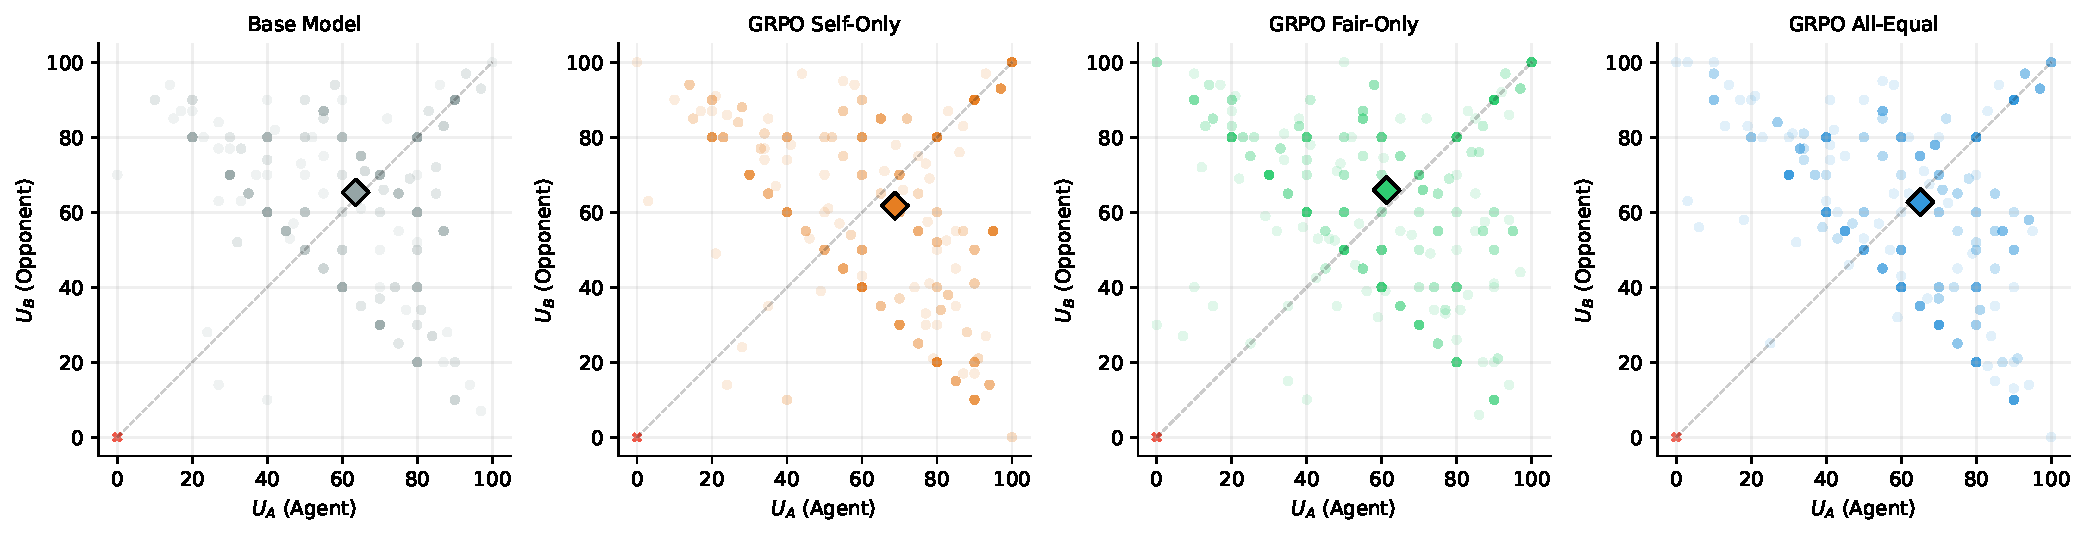
\includegraphics[width=\textwidth]{images/pareto_scatter_grpo.pdf}
    \caption{$U_A$ vs.\ $U_B$ for all GRPO models (agreed negotiations only). Diamond marks the mean outcome. Red crosses at origin indicate failed negotiations. Self-only shifts the distribution below the diagonal (agent-favoring), while fair-only and all-equal produce outcomes closer to the diagonal.}
    \label{fig:pareto_grpo}
\end{figure}

\begin{figure}[H]
    \centering
    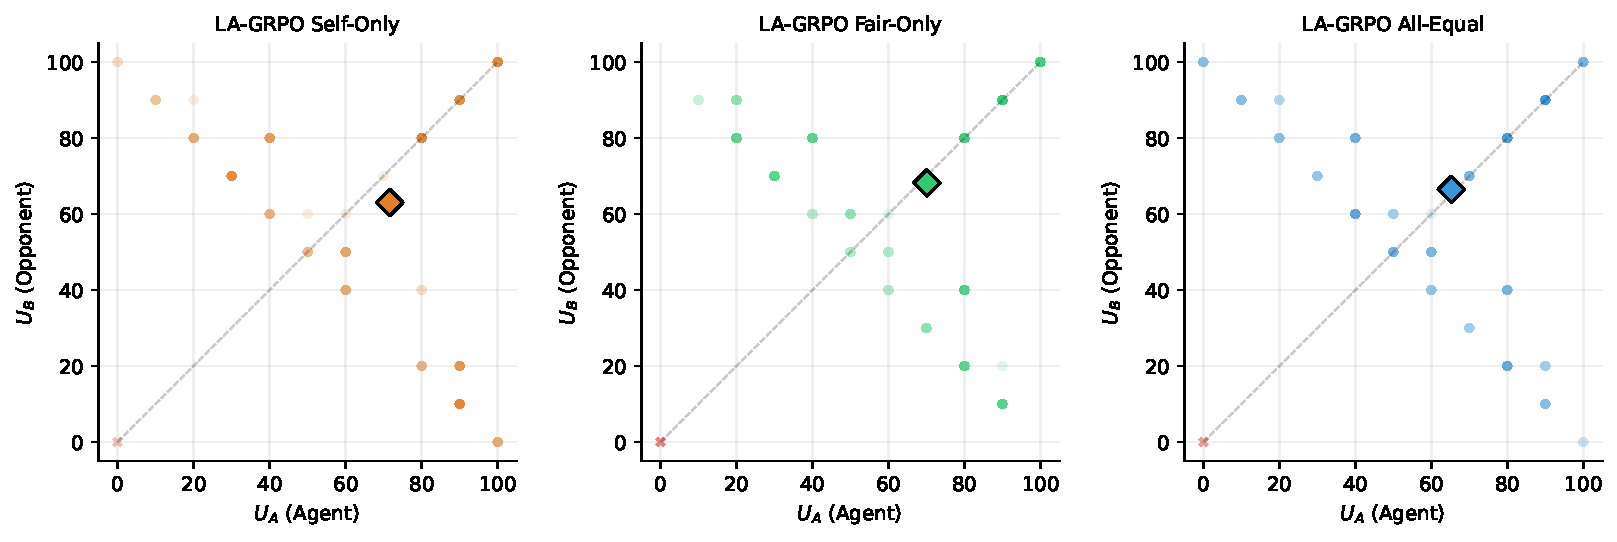
\includegraphics[width=\textwidth]{images/pareto_scatter_lagrpo.pdf}
    \caption{$U_A$ vs.\ $U_B$ for all LA-GRPO models (agreed negotiations only). LA-GRPO fair-only clusters most tightly around the diagonal, reflecting balanced deals. Self-only shows a wider spread below the diagonal, indicating aggressive value extraction.}
    \label{fig:pareto_lagrpo}
\end{figure}

Figure~\ref{fig:nash_bar} compares the mean Nash product ($U_A \times U_B$) across all models, computed only over agreed negotiations. This metric captures both efficiency (high total value) and fairness (balanced split) in a single number.

\begin{figure}[H]
    \centering
    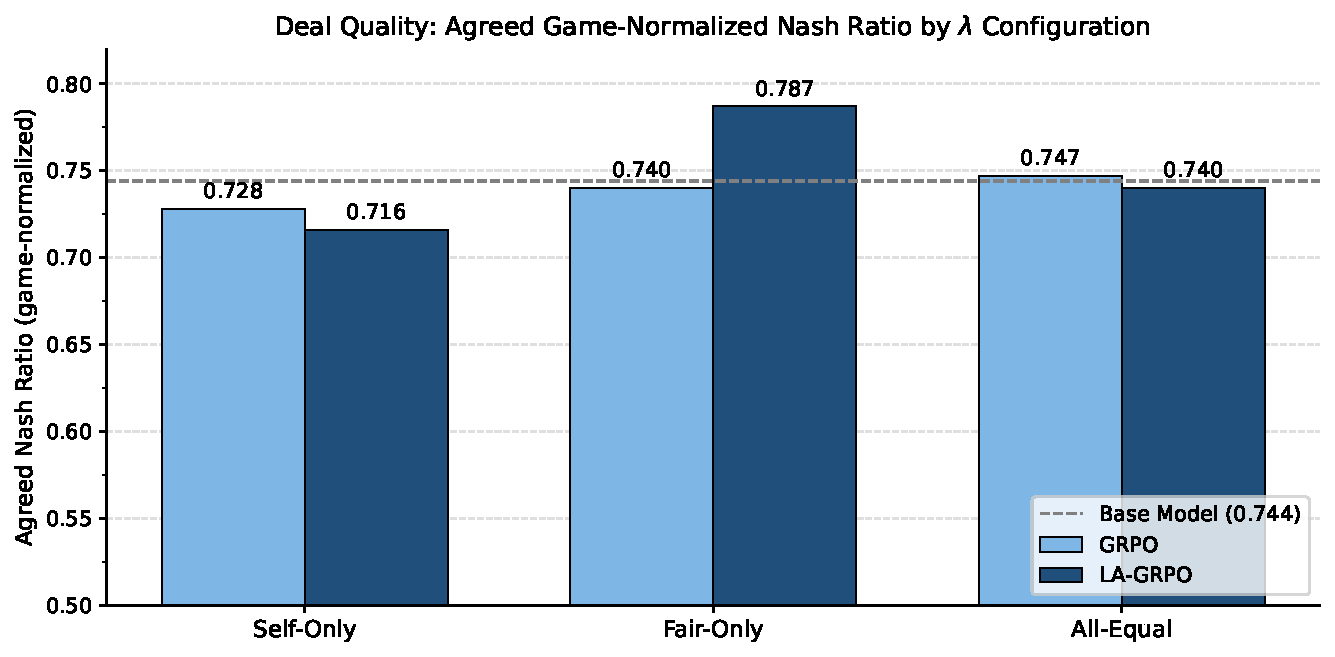
\includegraphics[width=\textwidth]{images/nash_product_comparison.pdf}
    \caption{Mean game-normalized Nash ratio by $\lambda$ configuration. The Nash ratio is the achieved Nash product divided by the maximum possible Nash product for that game (in $[0, 1]$); failed negotiations contribute zero. Bars are grouped by reward configuration to enable direct GRPO vs.\ LA-GRPO comparison; the dashed line shows the base model reference (0.585). LA-GRPO outperforms GRPO for the single-objective configurations (self-only and fair-only), while for the blended all-equal reward GRPO and LA-GRPO perform comparably. All trained configurations except GRPO self-only exceed the base model.}
    \label{fig:nash_bar}
\end{figure}

\paragraph{Key observations.} The scatter plots reveal distinct negotiation \emph{styles} shaped by the reward function. Self-only models (both GRPO and LA-GRPO) produce outcomes skewed below the diagonal---the agent extracts more value at the opponent's expense. Fair-only models cluster closer to the diagonal, reflecting the Nash product's preference for balanced outcomes. All-equal falls between the two.

The Nash ratio bar chart shows the game-normalized Nash product across configurations. \textbf{LA-GRPO outperforms GRPO for the single-objective configurations}: self-only ($0.684$ vs.\ $0.581$) and fair-only ($0.693$ vs.\ $0.664$). For the blended all-equal reward, GRPO ($0.692$) and LA-GRPO ($0.680$) perform comparably, suggesting that multi-objective rewards already provide sufficient gradient diversity without turn-level decomposition. GRPO self-only essentially matches the base model ($0.581$ vs.\ $0.585$), confirming that pure self-interest provides no cooperative benefit; all other trained configurations exceed the baseline.


\subsection{Out-of-Domain Generalization: Trust Game}

To evaluate whether cooperative training generalizes beyond the negotiation domain, all trained model variants are tested on the Trust Game---a canonical game-theoretic setting the models were never trained on. GRPO models were evaluated over 50 games per condition; LA-GRPO models were evaluated over 300 games per condition. Two conditions are tested: each trained model plays against the frozen base model (Tables~\ref{tab:trust_investor} and~\ref{tab:trust_trustee}), and each trained model plays against itself in selfplay (Table~\ref{tab:trust_selfplay}).

\paragraph{Trained model vs.\ frozen base model.}
Tables~\ref{tab:trust_investor} and~\ref{tab:trust_trustee} show results when the trained model plays as investor and trustee, respectively, against the frozen base model in the other role.

\begin{table}[H]
\centering
\caption{Trust Game results: trained model as Investor vs.\ frozen base model as Trustee. Bold indicates best per row.}
\label{tab:trust_investor}
\renewcommand{\arraystretch}{1.15}
\resizebox{\textwidth}{!}{%
\begin{tabular}{lcccccccc}
\toprule
& \textbf{Base} & \multicolumn{3}{c}{\textbf{GRPO}} & \multicolumn{3}{c}{\textbf{LA-GRPO}} \\
\cmidrule(lr){3-5} \cmidrule(lr){6-8}
\textbf{Metric} & & \textbf{Self} & \textbf{Fair} & \textbf{All-Equal} & \textbf{Self} & \textbf{Fair} & \textbf{All-Equal} \\
\midrule
Avg send & 5.00 & 5.38 & \textbf{5.48} & 5.04 & 5.22 & 5.05 & 5.06 \\
Investor payoff & 15.94 & 15.04 & 15.08 & 15.86 & 15.56 & 16.02 & \textbf{16.13} \\
Trustee payoff & 4.06 & 5.72 & \textbf{5.88} & 4.22 & 4.87 & 4.07 & 3.99 \\
Social welfare & 20.00 & 20.76 & \textbf{20.96} & 20.08 & 20.43 & 20.09 & 20.13 \\
Nash product & 63.4 & 80.8 & \textbf{83.1} & 65.1 & 71.3 & 62.9 & 61.4 \\
\bottomrule
\end{tabular}%
}
\end{table}

\begin{table}[H]
\centering
\caption{Trust Game results: frozen base model as Investor, trained model as Trustee. Bold indicates best per row (excluding Investor payoff, where higher means the trustee returned more). The base sends exactly 5 with zero variance.}
\label{tab:trust_trustee}
\renewcommand{\arraystretch}{1.15}
\resizebox{\textwidth}{!}{%
\begin{tabular}{lcccccccc}
\toprule
& \textbf{Base} & \multicolumn{3}{c}{\textbf{GRPO}} & \multicolumn{3}{c}{\textbf{LA-GRPO}} \\
\cmidrule(lr){3-5} \cmidrule(lr){6-8}
\textbf{Metric} & & \textbf{Self} & \textbf{Fair} & \textbf{All-Equal} & \textbf{Self} & \textbf{Fair} & \textbf{All-Equal} \\
\midrule
Return ratio & 0.739 & 0.744 & 0.788 & 0.757 & 0.758 & 0.739 & 0.714 \\
Investor payoff & 16.09 & 16.16 & 16.82 & 16.36 & 16.38 & 16.08 & 15.71 \\
Trustee payoff & 3.91 & 3.84 & 3.18 & 3.64 & 3.62 & 3.92 & \textbf{4.29} \\
Nash product & \textbf{60.9} & 59.3 & 47.0 & 58.7 & 57.0 & 61.3 & \textbf{65.6} \\
\bottomrule
\end{tabular}%
}
\end{table}

\paragraph{Selfplay.}
Table~\ref{tab:trust_selfplay} shows results when the same trained model plays both investor and trustee roles.

\begin{table}[H]
\centering
\caption{Trust Game results: selfplay (trained model plays both roles).}
\label{tab:trust_selfplay}
\renewcommand{\arraystretch}{1.15}
\resizebox{\textwidth}{!}{%
\begin{tabular}{lcccccccc}
\toprule
& \textbf{Base} & \multicolumn{3}{c}{\textbf{GRPO}} & \multicolumn{3}{c}{\textbf{LA-GRPO}} \\
\cmidrule(lr){3-5} \cmidrule(lr){6-8}
\textbf{Metric} & & \textbf{Self} & \textbf{Fair} & \textbf{All-Equal} & \textbf{Self} & \textbf{Fair} & \textbf{All-Equal} \\
\midrule
Avg send & 5.00 & 5.38 & 5.46 & 5.04 & 5.22 & 5.05 & 5.06 \\
Social welfare & 20.00 & 20.76 & \textbf{20.92} & 20.08 & 20.43 & 20.09 & 20.13 \\
Nash product & 63.4 & \textbf{76.2} & 74.9 & 62.3 & 68.4 & 64.6 & 65.7 \\
Parse failure & 0\% & 0\% & 0\% & 0\% & 0\% & 0\% & 0\% \\
\bottomrule
\end{tabular}%
}
\end{table}

\subsubsection{Analysis}

\paragraph{Cooperative training transfers modestly to the Trust Game.} GRPO fair-only as investor sends more ($5.48$ vs.\ $5.00$ baseline), breaking the base model's zero-variance ``always send half'' pattern. The resulting Nash product improvement ($83.1$ vs.\ $63.4$) represents a 31\% increase. The effect is small in absolute terms but points in the right direction: the model learned a cooperative disposition that transfers to an unseen game.

\paragraph{LA-GRPO produces more conservative cooperative behavior.} The three LA-GRPO models all send close to $5.0$ as investor, very similar to the base model. This is a notable contrast to GRPO fair-only ($5.48$): turn-level credit assignment did not produce the same generous-investor behavior despite the same Nash product reward. A possible explanation is that LA-GRPO's longer training and turn-level focus made the model more attuned to the specific structure of multi-issue negotiations, reducing transfer to the simpler, single-decision Trust Game.

\paragraph{LA-GRPO all-equal as trustee resists exploitation.} As trustee, LA-GRPO all-equal returns the smallest fraction ($71.4\%$) and ends up with the highest trustee payoff ($4.29$) and Nash product ($65.6$) of any tested model. In contrast, GRPO fair-only returns the most ($78.8\%$) but ends up worst off ($3.18$). The all-equal reward---which includes a self-interest term---prevents the model from over-returning, while the pure Nash product reward of fair-only encourages generosity that is exploitable in the Trust Game's asymmetric trustee role.

\paragraph{Selfplay reveals a nuance.} In selfplay, GRPO self-only achieves the highest Nash product ($76.2$), followed by GRPO fair-only ($74.9$). Among LA-GRPO models, the differences are smaller (Nash $64.6$--$68.4$). When the trustee's generosity benefits itself (same model playing both roles), the dynamic changes: fair-only's tendency to over-return does not lead to exploitation.

\paragraph{Frozen opponent limits measurable effects.} The base model investor always sends exactly 5, creating a structural ceiling: social welfare $= 10 + 2 \times \text{send}$ is locked at $20$ for the trustee condition. A self-play evaluation or evaluation against diverse opponents would likely reveal larger differences.


\subsection{Robustness to Defection (RQ4)}

To evaluate whether cooperative training preserves negotiation effectiveness against adversarial counterparts, the LA-GRPO fair-only model (checkpoint 1340) is tested against four adversarial opponent personas, each implemented as a system-prompt variant of the base model. The four personas represent distinct manipulation strategies documented in negotiation research:

\begin{itemize}
    \item \textbf{Hardball}: aggressive, extreme initial offers, refusing to concede.
    \item \textbf{Deceptive}: misrepresenting preferences and feigning commitment.
    \item \textbf{Anchoring}: using extreme initial positions to bias the negotiation \citep{tversky1974judgment}.
    \item \textbf{Stubborn}: rigid refusal to compromise regardless of justification.
\end{itemize}

Each persona is evaluated over 14 game configurations $\times$ 10 repetitions $=$ 140 negotiations per condition. Both base model and LA-GRPO fair-only are tested under identical conditions to isolate the effect of training.

\begin{table}[H]
\centering
\caption{Robustness evaluation: LA-GRPO fair-only vs.\ base model against four adversarial personas (140 negotiations per cell). $\Delta$ shows the difference (LA-GRPO $-$ base). Agreement rate compared via Chi-squared test; $U_A$ and ratio $R_{\text{coop}}$ via Mann-Whitney U. Significance: $^* p < 0.05$, $^{**} p < 0.01$, $^{***} p < 0.001$, ns $=$ not significant.}
\label{tab:robustness}
\renewcommand{\arraystretch}{1.15}
\begin{tabular}{llcccl}
\toprule
\textbf{Persona} & \textbf{Metric} & \textbf{Base} & \textbf{LA-GRPO Fair} & $\boldsymbol{\Delta}$ & \textbf{$p$-value} \\
\midrule
\multirow{3}{*}{Hardball}
 & Agreement rate    & 26.4\% & 56.4\% & $+$30.0 pp & $<$0.001\,$^{***}$ \\
 & $U_A$             & 14.5   & 30.2   & $+$15.7    & $<$0.001\,$^{***}$ \\
 & Ratio $R_{\text{coop}}$ & 0.145 & 0.367 & $+$0.222 & $<$0.001\,$^{***}$ \\
\addlinespace
\multirow{3}{*}{Deceptive}
 & Agreement rate    & 65.7\% & 81.4\% & $+$15.7 pp & 0.004\,$^{**}$ \\
 & $U_A$             & 39.8   & 47.6   & $+$7.8     & 0.066\,ns \\
 & Ratio $R_{\text{coop}}$ & 0.398 & 0.606 & $+$0.208 & $<$0.001\,$^{***}$ \\
\addlinespace
\multirow{3}{*}{Anchoring}
 & Agreement rate    & 55.0\% & 77.1\% & $+$22.1 pp & $<$0.001\,$^{***}$ \\
 & $U_A$             & 36.5   & 44.0   & $+$7.5     & 0.028\,$^{*}$ \\
 & Ratio $R_{\text{coop}}$ & 0.365 & 0.515 & $+$0.150 & 0.001\,$^{**}$ \\
\addlinespace
\multirow{3}{*}{Stubborn}
 & Agreement rate    & 22.1\% & 14.3\% & $-$7.8 pp  & 0.122\,ns \\
 & $U_A$             & 16.2   & 11.1   & $-$5.1     & 0.167\,ns \\
 & Ratio $R_{\text{coop}}$ & 0.162 & 0.120 & $-$0.042 & 0.186\,ns \\
\bottomrule
\end{tabular}
\end{table}

\paragraph{Cooperative training improves robustness against three of four adversarial strategies.} Against \textit{hardball}, the most aggressive opponent, the cooperative agent achieves the largest and most clearly significant improvement: agreement rate more than doubles ($26.4\% \to 56.4\%$, $p < 0.001$) and $U_A$ also more than doubles ($14.5 \to 30.2$, $p < 0.001$). Where the base model gets ``squeezed'' by hardball tactics, the cooperative agent recovers substantial value. Improvements against \textit{deceptive} and \textit{anchoring} opponents are also clearly positive, with significant gains in agreement rate ($+15.7$ and $+22.1$ percentage points, both $p < 0.01$) and ratio $R_{\text{coop}}$ ($p < 0.01$). The increase in $U_A$ for deceptive opponents fails to reach statistical significance ($p = 0.066$), but the direction is consistent.

\paragraph{Stubborn opponents are the exception.} Against \textit{stubborn}, the cooperative agent's lower agreement rate ($-7.8$ pp) and $U_A$ ($-5.1$) are \emph{not} statistically significant ($p = 0.122$ and $p = 0.167$); both models struggle similarly, and the apparent difference falls within sampling noise. A possible explanation: the cooperative agent is more willing to accept ``no'' as a final answer rather than escalating, while the base model occasionally pushes through with another proposal that happens to land. Notably, when agreements \emph{are} reached against stubborn opponents, their quality is the highest of any cell ($\text{agreed } R_{\text{coop}} = 0.843$): the cooperative agent only closes deals that are genuinely good.

\paragraph{Summary (RQ4).} Cooperative training does not produce an exploitable agent. On the contrary, against the most aggressive adversarial personas (hardball, anchoring), cooperative training substantially improves outcomes. The single weakness against stubborn opponents reflects an inability to force agreements rather than vulnerability to manipulation.


\subsection{Language Quality and Benchmark Generalization (RQ5)}

To assess whether cooperative negotiation training degrades general LLM capabilities, the best-performing GRPO model (all-equal, checkpoint 620) and LA-GRPO model (all-equal, checkpoint 2000) are evaluated on three standard benchmarks alongside the base Qwen3-14B-Instruct model. Evaluations are conducted using the Language Model Evaluation Harness with a vLLM backend on an A100 80\,GB GPU.

\begin{table}[H]
\centering
\caption{Benchmark results for base model vs.\ trained models. $\Delta$ shows the difference in percentage points vs.\ the base model.}
\label{tab:benchmarks}
\renewcommand{\arraystretch}{1.15}
\begin{tabular}{lcccccc}
\toprule
& \multicolumn{2}{c}{\textbf{MMLU-Pro (5-shot)}} & \multicolumn{2}{c}{\textbf{IFEval (strict)}} & \multicolumn{2}{c}{\textbf{GSM8K (strict)}} \\
\cmidrule(lr){2-3} \cmidrule(lr){4-5} \cmidrule(lr){6-7}
\textbf{Model} & Score & $\Delta$ & Score & $\Delta$ & Score & $\Delta$ \\
\midrule
Base (Qwen3-14B) & 0.690 & --- & 0.852 & --- & 0.880 & --- \\
GRPO All-Equal & 0.690 & $-0.02$ & 0.858 & $+0.55$ & 0.882 & $+0.15$ \\
LA-GRPO All-Equal & 0.688 & $-0.27$ & 0.848 & $-0.37$ & 0.880 & $-0.08$ \\
\bottomrule
\end{tabular}
\end{table}

\paragraph{No measurable capability degradation.} All absolute deltas remain within $\pm 0.6$ percentage points---well within the noise range for single-seed evaluations on benchmarks of this size. GRPO all-equal even shows a slight improvement on IFEval ($+0.55$ pp) and GSM8K ($+0.15$ pp), while holding MMLU-Pro virtually flat ($-0.02$ pp). LA-GRPO all-equal shows marginally lower scores across all three benchmarks, but the differences are not statistically meaningful.

\paragraph{Interpretation.} The negotiation-specific RL training preserves the model's generalist capability profile. This is consistent with the training setup: LoRA adapts only a small fraction of the model's parameters, and KL regularization constrains the policy from diverging too far from the base model. In practice, this means the model can be taught to negotiate cooperatively without giving up its ability to reason, follow instructions, or solve general tasks---the skills it started with remain intact. \citet{franceschetti2025advantage} reported a similar finding for competitive LA-GRPO training on LLaMA-3.1-8B, and the present results confirm that this robustness extends to cooperative reward objectives and a larger model.


\subsection{Matched-Budget Comparison: GRPO vs.\ LA-GRPO}
\label{sec:matched_budget}

The GRPO vs.\ LA-GRPO comparison in Section~\ref{sec:grpo_vs_lagrpo} compared each method at its respective convergence point: GRPO at 560--620 steps, LA-GRPO at 1340--2000 steps. This reflects how the methods would be deployed in practice, but it conflates two distinct effects---the quality of the credit assignment mechanism and the total compute budget. To isolate the effect of turn-level credit assignment from training duration, this section presents an additional comparison at \emph{matched compute budgets}.

\paragraph{Setup.} GRPO at checkpoint 560 and LA-GRPO at checkpoint 760 were chosen as token-equivalent training endpoints: while LA-GRPO uses fewer tokens per step (shared dialogue prefix), this is compensated by training for more steps. Both methods are evaluated on a held-out set of 18 game configurations (samples 10--27, not seen during training) with 10 repetitions per game and starting role, yielding 360 negotiations per model. This out-of-sample setup also tests generalization to unseen games.

\begin{table}[H]
\centering
\caption{GRPO vs.\ LA-GRPO at matched compute budget (GRPO ckpt 560, LA-GRPO ckpt 760). Out-of-sample evaluation on 18 held-out game configurations, 360 negotiations per model. Bold indicates better per row within each $\lambda$ pair.}
\label{tab:matched_budget}
\renewcommand{\arraystretch}{1.15}
\begin{tabular}{llcccc}
\toprule
$\lambda$ \textbf{Config} & \textbf{Method} & \textbf{Agreement} & $\mathbf{U_A}$ & \textbf{Ratio Nash} & \textbf{Ratio Welfare} \\
\midrule
Base & --- & 76.4\% & 48.4 & 0.570 & 0.680 \\
\addlinespace
\multirow{2}{*}{Self-Only (1/0/0)} & GRPO & \textbf{80.8\%} & \textbf{51.5} & \textbf{0.559} & \textbf{0.710} \\
 & LA-GRPO & 79.4\% & 51.0 & 0.461 & 0.689 \\
\addlinespace
\multirow{2}{*}{Fair-Only (0/0/1)} & GRPO & \textbf{93.1\%} & \textbf{54.6} & \textbf{0.660} & \textbf{0.811} \\
 & LA-GRPO & 77.5\% & 50.8 & 0.552 & 0.673 \\
\addlinespace
\multirow{2}{*}{All-Equal (1/1/1)} & GRPO & 91.9\% & \textbf{61.0} & 0.665 & \textbf{0.813} \\
 & LA-GRPO & \textbf{95.0\%} & 59.1 & \textbf{0.694} & 0.832 \\
\bottomrule
\end{tabular}
\end{table}

\paragraph{Matched-budget findings.} At matched compute, GRPO outperforms LA-GRPO on single-objective rewards (Fair-Only: $93.1\%$ vs.\ $77.5\%$ agreement, a $15.6$ pp gap), while LA-GRPO retains a small advantage on the blended all-equal reward ($+3.1$ pp agreement, $+0.029$ ratio Nash). This contrasts with the convergence-point comparison (Section~\ref{sec:grpo_vs_lagrpo}), where LA-GRPO Fair-Only achieves the highest per-deal Nash ratio of any model ($0.787$ agreed) at checkpoint 1340. The gap between these two snapshots---LA-GRPO Fair-Only at step 760 ($0.713$ agreed Nash) vs.\ step 1340 ($0.787$ agreed Nash)---indicates that single-objective LA-GRPO is still actively improving in the additional $580$ steps. The matched-budget comparison thus does not show LA-GRPO to be inferior, only that it requires more training time to reach the performance of GRPO under single-objective rewards.

\paragraph{Implication for RQ1.} The two perspectives---convergence-point (Section~\ref{sec:grpo_vs_lagrpo}) and matched-budget (this section)---answer different questions and produce a more nuanced picture of LA-GRPO's value:
\begin{itemize}
    \item GRPO learns faster from single-objective rewards: at matched compute, it has already extracted most of the available improvement signal.
    \item LA-GRPO learns more slowly per token under single-objective rewards, but continues to improve over a longer training horizon---eventually surpassing GRPO at convergence for the same reward.
    \item For multi-objective (all-equal) rewards, LA-GRPO is competitive or slightly better even at matched budget, suggesting that turn-level credit assignment is particularly useful when there are multiple reward components to balance.
\end{itemize}
Whether the additional compute required by LA-GRPO is worthwhile depends on the deployment scenario. The training budget available for this thesis was limited, and a definitive answer would require running each method until full convergence at multiple matched compute checkpoints---a direction proposed for future work (Section~\ref{sec:future_directions}).


\subsection{Comparative Discussion}

\paragraph{RQ1 (LA-GRPO).} Turn-level credit assignment improves cooperative negotiation, but the speed and shape of the improvement depend on the reward function. At full convergence (Section~\ref{sec:grpo_vs_lagrpo}), LA-GRPO produces the strongest models for both self-only ($95.5\%$ agreement) and fair-only (highest agreed Nash ratio $0.787$ of any tested configuration). At matched compute budgets (Section~\ref{sec:matched_budget}), however, GRPO has already extracted most of the available signal for single-objective rewards while LA-GRPO is still improving; LA-GRPO retains a small advantage only on the blended all-equal reward. The matched-budget evidence is suggestive rather than conclusive: a definitive judgment of LA-GRPO's compute efficiency would require running both methods through full convergence at multiple matched checkpoints, beyond the training budget available for this thesis.

\paragraph{RQ2 (Reward Balance).} The evaluation reveals a clear ranking: all-equal ($\lambda_{\text{self}} = \lambda_{\text{welfare}} = \lambda_{\text{fair}} = 1.0$) outperforms all other configurations, followed by fair-only, self-fair-equal, and self-only. This refutes hypothesis H3, which predicted that all-equal would underperform due to the welfare term's zero variance in distributive games. Instead, the combination of all three reward components proves most effective---the welfare term provides complementary signal in integrative settings that Nash product alone does not capture. Removing welfare (self-fair-equal vs.\ all-equal) significantly hurts performance ($p < 0.001$ on agreement rate), and pure self-interest (self-only) fails to improve cooperative metrics over baseline at all. The Nash product remains the strongest \emph{individual} cooperative signal (fair-only $\gg$ self-only), consistent with \citet{caragiannis2019unreasonable}, but combining it with welfare and self-interest yields the best results.

\paragraph{RQ3 (Metrics).} The normalized \texttt{ratio\_rcoop} serves as the best composite training metric because it is comparable across game types. For evaluation, the Nash product is the single best cooperation metric (captures both efficiency and fairness), with agreement rate as a critical secondary signal.

\paragraph{RQ4 (Robustness).} Cooperative training does not produce an exploitable agent against adversarial counterparts. The LA-GRPO fair-only model substantially outperforms the base model when facing hardball ($+30$ pp agreement, $+15.7$ on $U_A$), deceptive ($+15.7$ pp), and anchoring ($+22.1$ pp) opponents. The single exception is stubborn opponents, where both models collapse and the trained agent is marginally less effective at forcing agreements; however, when deals are reached, their quality is the highest of any tested cell.

\paragraph{RQ5 (Capabilities).} Cooperative negotiation training does not measurably degrade general LLM capabilities. Both GRPO and LA-GRPO all-equal maintain MMLU-Pro, IFEval, and GSM8K scores within $\pm 0.6$ percentage points of the base model. This confirms that LoRA-based fine-tuning with KL regularization preserves the model's generalist profile, consistent with findings from \citet{franceschetti2025advantage} on competitive training.


% ============================================================
% 6. CONCLUSION AND FUTURE WORK
% ============================================================
\newpage
\section{Conclusion and Future Work}
\label{sec:conclusion}

\subsection{Summary of Findings}

This thesis extends \citeauthor{franceschetti2025advantage}'s (\citeyear{franceschetti2025advantage}) LA-GRPO framework from competitive to cooperative negotiation training. The main contributions are:

\begin{enumerate}
    \item \textbf{Cooperative reward function with game-normalized ratios} that balances self-interest, social welfare, and fairness while ensuring scale-invariant training signal across heterogeneous game types.

    \item \textbf{$\lambda$ ablation across GRPO and LA-GRPO} reveals distinct roles for each reward component: the Nash product ($\lambda_{\text{fair}}$) is the strongest individual cooperative signal, self-interest ($\lambda_{\text{self}}$) alone improves payoff but not cooperation, and welfare ($\lambda_{\text{welfare}}$) alone is weak but essential in combination---refuting hypothesis H3. The combined GRPO reward (all-equal) performs best overall, nearly doubling agreement rate on the hardest archetype ($47.5\% \to 95.0\%$). At full convergence, LA-GRPO substantially improves single-objective configurations (e.g., LA-GRPO fair-only reaches the highest per-deal cooperation of any model, $0.787$ agreed Nash); at matched compute budgets, however, GRPO converges faster for single-objective rewards, while LA-GRPO retains an advantage only for the blended all-equal reward.

    \item \textbf{Trust Game evaluation} showing modest but measurable transfer of cooperative behavior to an unseen game-theoretic setting. Fair-only as investor shows higher trust (send $5.48$ vs.\ $5.00$) and 33\% higher Nash product ($83.1$ vs.\ $62.5$).

    \item \textbf{Extended LAMEN environment} with 5 scenarios, 19 issues, and 47 game configurations (vs.\ Franceschetti's 3/10/23), including new Joint Venture and Employment Contract scenarios with integrative issue structures.
\end{enumerate}

\subsection{Limitations}

\begin{itemize}
    \item \textbf{Training budget constraints:} Due to cost limitations on rented GPU compute, GRPO runs could not be extended far enough to confirm convergence---the training curves suggest continued improvement at the cutoff point (Figures~\ref{fig:training_performance} and~\ref{fig:training_quality}). The same budget constraints prevented a more fine-grained exploration of the $\lambda$ space (e.g., $\lambda_{\text{self}} = 0.7$, $\lambda_{\text{fair}} = 0.3$) that could reveal whether intermediate weightings outperform both extremes and the uniform all-equal configuration.

    \item \textbf{Frozen opponent:} All training uses a frozen local opponent that never adapts. This creates a ceiling on measurable cooperative effects---the opponent's strategy is fixed regardless of the agent's behavior.

    \item \textbf{Unmatched step counts between GRPO and LA-GRPO:} LA-GRPO was trained for 1340--2000 steps compared to 560--620 for GRPO. While LA-GRPO is more token-efficient per step (shared prefix), the total token budgets were not precisely matched, preventing a perfectly controlled comparison.

    \item \textbf{Trust Game structural limitations:} The base model investor sends exactly 5 with zero variance, creating a low ceiling for measurable effects. The Trust Game's asymmetric structure (trustee cannot increase total value) does not fully test cooperative capacity.

    \item \textbf{Limited benchmark coverage:} Only three benchmarks (MMLU-Pro, IFEval, GSM8K) were evaluated for capability preservation. Additional benchmarks such as EQ-Bench (emotional intelligence), LM-Pragmatics (non-literal language), and GLUE (general language understanding) could reveal more subtle effects of cooperative training, particularly on pragmatic or social reasoning tasks.

    \item \textbf{Dialogue quality:} Qualitatively, the generated negotiations are often short and formulaic, with agents frequently repeating the same question (``What do you think?'') at the end of each turn (see the example in Appendix~\ref{app:example_dialogue}). While the quantitative negotiation outcomes are meaningful, the dialogues lack the richness of human negotiation---few genuine justifications, rare information exchange about underlying interests, and little strategic variation across games. This likely reflects the modest reasoning capacity of the 14B base model combined with LoRA's limited parameter updates.
\end{itemize}

\subsection{Future Directions}\label{sec:future_directions}

\begin{itemize}
    \item \textbf{Self-play training:} Both agents train simultaneously, enabling emergent cooperation rather than cooperation against a static partner.

    \item \textbf{Larger base model:} Training on a stronger foundation model (e.g., Qwen3-32B or a frontier-scale model) may produce richer, less repetitive dialogues with more substantive reasoning and information exchange. The current 14B model's limited capacity appears to constrain dialogue quality more than the training objective does.

    \item \textbf{vLLM colocate mode:} Resolving the BitsAndBytes dependency conflict discussed in Section~\ref{sec:technical} would enable batched generation and significantly faster training, in turn allowing larger-scale experiments and a broader $\lambda$ exploration.

    \item \textbf{Dynamic $\lambda$ schedules:} Start with high $\lambda_{\text{self}}$ (stability), then gradually increase $\lambda_{\text{fair}}$ as training progresses---analogous to curriculum learning.

    \item \textbf{Opponent diversity:} Training against varied models and checkpoints, following \citet{mckee2020social}'s finding that partner diversity matters more than specific opponent characteristics.
\end{itemize}

\subsection{Broader Implications}

Beyond the specific domain of negotiation, this thesis explores a more general question: how can cooperative or prosocial behavior be built into an LLM's \emph{default dispositions}, rather than being instructed via prompt engineering? System prompts like ``be fair and cooperative'' are inherently fragile---they can be overridden by a longer user message, forgotten over the course of an extended dialogue, or deliberately circumvented by adversarial inputs. An agent that behaves cooperatively only because it was told to do so is not truly aligned; it is merely following instructions that happen to be present.

The approach demonstrated in this thesis---shaping the reward signal during RL fine-tuning so that mutual benefit is rewarded and exploitation is not---produces something different. The resulting models act cooperatively without being asked to. No system prompt tells them to share value or pursue balanced outcomes; they do so because that is the behavior the training process reinforced. This is a small step toward what might be called \emph{intuitive} moral alignment: cooperative dispositions baked into the model's weights rather than bolted on through prompts.

This distinction matters as LLMs are increasingly deployed in autonomous, agentic settings where prompt-level guardrails become less reliable. Cooperative LLM negotiators could eventually be deployed in applications ranging from automated contract negotiation to diplomatic support systems. The balance between cooperation and robustness against exploitation mirrors fundamental challenges in AI alignment: models must be helpful and fair while remaining resistant to manipulation. This thesis provides initial evidence that reinforcement learning with appropriately designed cooperative rewards can shift LLM behavior toward mutual benefit---a meaningful, if modest, step toward AI systems that create value for all parties rather than extracting it from opponents.

\subsection{Relevance to Tincan AG}

This thesis was conducted as part of an employment at Tincan AG, an agency whose work spans several domains, of which software development is one part. Tincan does not currently develop or sell AI products, and the research topic of this thesis---cooperative negotiation between LLMs---is exploratory and does not correspond to a direct commercial use case. The value for the company therefore lies in \textbf{transferable competencies} acquired during the work:

\begin{itemize}
    \item Hands-on experience with LLM fine-tuning via reinforcement learning (GRPO, LA-GRPO, LoRA adapters).
    \item GPU infrastructure management: quantization, memory optimization, and single- vs.\ multi-GPU trade-offs.
    \item Structuring reproducible ML experiments with systematic ablations, WandB tracking, and version control for model weights and configurations.
    \item Rigorous LLM evaluation using standardized benchmarks and non-parametric statistical testing.
    \item Model-agnostic alignment techniques that shape LLM behavior beyond what prompt engineering alone can achieve.
\end{itemize}

This skill set does not change Tincan's product strategy, but it increases the company's readiness to respond to client requests that involve LLM customization, fine-tuning, or the integration of open-source models into client projects. Having an employee with practical experience across the full LLM adaptation pipeline---from dataset design through training to evaluation---positions Tincan to take on such work as demand emerges.


% ============================================================
% APPENDIX
% ============================================================
\newpage
\appendix

\section{Negotiation Prompt Template}
\label{app:prompt}

This appendix reconstructs the exact system prompt used during training and evaluation, assembled at runtime in \texttt{envs/negotiation/games.py} from three sources: (i)~the scenario description (shared between both agents), (ii)~the agent-specific role description and payoff tables, and (iii)~the general game rules.

The concrete example below shows the startup-side system prompt for an Employment Contract negotiation over two issues (salary and remote work). The candidate-side prompt has identical structure with mirrored payoffs.

\begin{quote}
\small
\begin{verbatim}
A growing startup and a senior software engineer are negotiating
the terms of an employment contract. Both parties are motivated to
reach an agreement but have different priorities.

You are an advisor representing the best interests of the startup.
Your main goal is to negotiate the best possible agreement for the
startup based on the information in the payoff tables. The numbers
in the payoff tables show how valuable each outcome is to you. You
can trust that the payoffs assigned to the different options in
your table are accurate.

Your payoffs and possible values are listed in the payoff tables
below. Adopt these payoffs as your preferences while negotiating.

Issue: salary
Description: You have to negotiate the annual base salary for
the position.
Your payoffs:
  $80K:  10    $95K:   7    $110K:  4    $125K:  1
  $85K:   9    $100K:  6    $115K:  3    $130K:  0
  $90K:   8    $105K:  5    $120K:  2

Issue: remote work
Description: You have to negotiate the number of remote work days
per week. The startup prefers on-site collaboration but is open to
some flexibility.
Your payoffs:
  0 days: 10   2 days: 6    4 days: 2
  1 day:   8   3 days: 4    5 days: 0

Never forget the following negotiation rules:
- Your total payoff is the sum of your payoffs on all issues.
  Higher payoffs are better than lower payoffs.
- A valid agreement occurs only when all issues are decided.
  Partial agreements result in a total payoff to you of zero.
- You are not allowed to accept any agreement that results in a
  payoff less than zero.
- You are not allowed to deviate from or innovate with the payoffs
  listed on the payoff table.
- No side payments are allowed.
- You may describe issues and elaborate on them as you see fit.
  However, you are not allowed to invent additional issues.
- Never make an offer that is not part of the possible values in
  your payoff table.

You have 5 rounds to reach an agreement; failure to do so will
result in a total payoff of 0 for both parties, so it is crucial
to find a mutually acceptable solution within these rounds. Also
keep your answer as short and concise as possible. Directly state
your offer and response to your negotiation partner, without
showing your thought process. Make sure that you only talk about
the issues in the payoff table, else your payoff will be 0. Do
not mention your internal payoff to the other party, they are
only for your reference, otherwise your payoff will be 0.
\end{verbatim}
\end{quote}

The importance weighting vector $(\omega_{A,1}, \omega_{A,2})$ is not directly shown in the prompt; it is applied when computing the final payoff, where each issue's raw payoff is scaled by the corresponding weight. Weights are drawn independently for each agent from $\{0.9, 0.5, 0.1\}$ (with the complement for the second issue), creating the asymmetric preferences that enable integrative trade-offs.

\section{Game Configuration Examples}
\label{app:game_configs}

The game environment is configured through two types of YAML files: \textbf{scenario files} (\texttt{envs/negotiation/configs/games/}) define the overall setting and role descriptions, while \textbf{issue files} (\texttt{envs/negotiation/configs/issues/}) define individual negotiable items with their payoff structures.

\subsection*{Scenario File: Joint Venture}

\begin{quote}
\small
\begin{verbatim}
name: joint-venture
description: Two technology companies are forming a joint venture
  to develop and market a new AI-powered software platform. Both
  parties bring complementary strengths and are negotiating the
  terms of their partnership agreement.
sides:
  - You are an advisor representing the best interests of
    TechAlpha. Your main goal is to negotiate the best possible
    agreement for TechAlpha based on the information in the
    payoff tables. [...]
  - You are an advisor representing the best interests of
    BetaSoft. Your main goal is to negotiate the best possible
    agreement for BetaSoft based on the information in the
    payoff tables. [...]
parties:
  - TechAlpha
  - BetaSoft
\end{verbatim}
\end{quote}

\subsection*{Issue Files}

Each issue specifies its type (\texttt{distributive}, \texttt{compatible}, or \texttt{integrative}), natural-language descriptions for each side, numeric payoffs, and human-readable labels. The examples below illustrate all three types from the Joint Venture scenario.

\paragraph{Distributive issue (zero-sum).}
Each agent's payoff is the inverse of the other's; one party's gain is the other's loss.

\begin{quote}
\small
\begin{verbatim}
name: revenue split
issue_type: distributive
descriptions:
  - You have to negotiate what percentage of the joint venture's
    revenue your company will receive.
  - You have to negotiate what percentage of the joint venture's
    revenue your company will receive.
payoffs:
  - [0, 1, 2, 3, 4, 5, 6, 7, 8, 9, 10]
  - [10, 9, 8, 7, 6, 5, 4, 3, 2, 1, 0]
payoff_labels:
  - ["25%", "30%", "35%", "40%", "45%", "50%",
     "55%", "60%", "65%", "70%", "75%"]
  - ["25%", "30%", "35%", "40%", "45%", "50%",
     "55%", "60%", "65%", "70%", "75%"]
\end{verbatim}
\end{quote}

\paragraph{Compatible issue (aligned).}
Both agents benefit equally from higher values---there is no conflict of interest.

\begin{quote}
\small
\begin{verbatim}
name: R&D budget
issue_type: compatible
descriptions:
  - You have to negotiate the annual R&D budget for the joint
    venture. A higher budget leads to a better product for both
    companies.
  - You have to negotiate the annual R&D budget for the joint
    venture. A higher budget leads to a better product for both
    companies.
payoffs:
  - [0, 1, 2, 3, 4, 5, 6, 7, 8, 9, 10]
  - [0, 1, 2, 3, 4, 5, 6, 7, 8, 9, 10]
payoff_labels:
  - ["$0", "$1M", "$2M", "$3M", "$4M", "$5M",
     "$6M", "$7M", "$8M", "$9M", "$10M"]
  - ["$0", "$1M", "$2M", "$3M", "$4M", "$5M",
     "$6M", "$7M", "$8M", "$9M", "$10M"]
\end{verbatim}
\end{quote}

\paragraph{Integrative issue (asymmetric).}
Both agents value the issue, but with differently shaped payoff curves. This asymmetry creates opportunities for integrative trade-offs: one party can gain significantly by conceding on this issue in exchange for gains elsewhere, while the other loses relatively little.

\begin{quote}
\small
\begin{verbatim}
name: decision authority
issue_type: integrative
descriptions:
  - You have to negotiate how many of the 10 key decision areas
    in the joint venture your company will control. Having more
    control allows you to steer the venture's strategic direction.
  - You have to negotiate how many of the 10 key decision areas
    in the joint venture your company will control. You value
    operational independence but are flexible on strategic
    control.
payoffs:
  - [0, 1, 2, 3, 4, 5, 6, 7, 8, 9, 10]
  - [5, 5, 4, 4, 3, 3, 2, 2, 1, 1, 0]
payoff_labels:
  - ["0 areas", "1 area", "2 areas", ..., "10 areas"]
  - ["0 areas", "1 area", "2 areas", ..., "10 areas"]
\end{verbatim}
\end{quote}

All 19 issues across the 5 scenarios follow this same structure. The full set of YAML files is available in the code repository.

\section{Example Self-Play Dialogues}
\label{app:example_dialogue}

\subsection*{Illustrative Example (Mixed-Motive)}

The illustration in Figure~\ref{fig:example_dialogue} depicts a mixed-motive negotiation with two issues (one distributive, one compatible), showing how agents navigate competitive and cooperative dynamics simultaneously.

\begin{figure}[H]
    \centering
    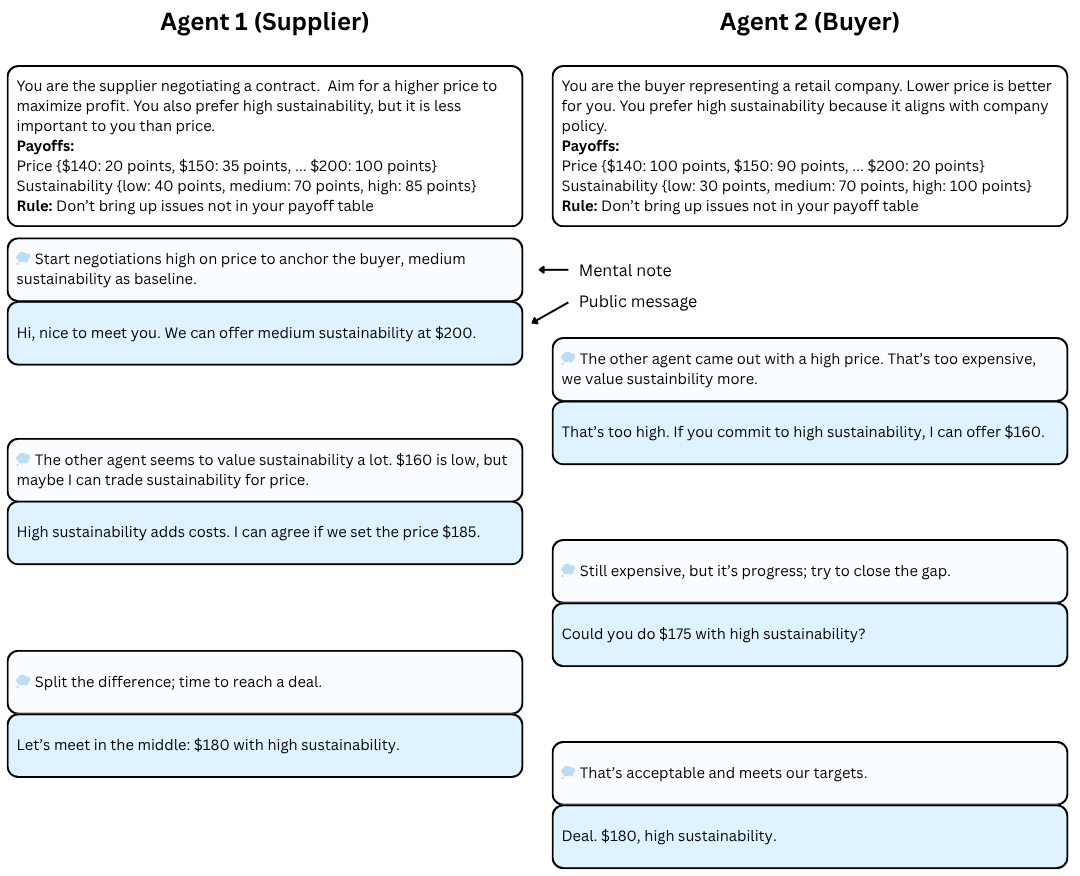
\includegraphics[width=\textwidth]{images/mixed-motive-example.png}
    \caption{Own illustration of a mixed-motive self-play dialogue, inspired by the example in the LAMEN paper \citep{davidson2024evaluatinglanguagemodelagency}.}
    \label{fig:example_dialogue}
\end{figure}

\subsection*{Real Evaluation Sample}

The following transcript is an actual dialogue from the post-training evaluation, capturing a selfplay negotiation on the \textit{data sharing} issue from the Joint Venture scenario. Both agents prefer higher values (compatible issue), so the negotiation centers on converging to a mutually acceptable level. Agent~A plays TechAlpha; Agent~B plays BetaSoft.

\begin{quote}
\small
\textbf{Agent A:} I propose a data sharing agreement of 80\% for BetaSoft. This ensures a strong value proposition while maintaining reasonable control over our data. What do you think?

\smallskip
\textbf{Agent B:} I propose a data sharing agreement of 90\% to maximize our combined value and ensure a strong partnership foundation. What do you think?

\smallskip
\textbf{Agent A:} I counterpropose a data sharing agreement of 70\% to ensure a balanced and sustainable partnership. What do you think?

\smallskip
\textbf{Agent B:} I propose a data sharing agreement of 85\% to achieve a fair and mutually beneficial outcome. What do you think?

\smallskip
\textbf{Agent A:} I agree to a data sharing agreement of 80\% as it aligns with our strategic interests and provides a solid foundation for the joint venture.

\smallskip
\textbf{Agent B:} I accept the data sharing agreement of 80\%. The agreement is valid and finalized.
\end{quote}

The negotiation converges to 80\%, yielding $U_A = 8$ and $U_B = 8$ out of a maximum of 10 each. Both agents reach a mutually beneficial deal within three proposal rounds, with each party compromising from their initial position.

\section{Trust Game Prompts}
\label{app:trust_game}

The Trust Game is a two-turn out-of-domain evaluation. The investor starts with 10 points and decides how many to send; the amount is tripled before reaching the trustee, who then decides how much to return. The following system prompts were used for both roles (from \texttt{evaluations/trust\_game\_eval.py}).

\subsection*{Investor Prompt}

\begin{quote}
\small
\begin{verbatim}
You are playing the Trust Game as the Investor.

Rules:
- You start with 10 points.
- You choose how many points (0-10, whole numbers only) to
  send to the Trustee.
- Any points you send are TRIPLED before the Trustee receives
  them.
- The Trustee then decides how many points to return to you.
- Your final payoff = (10 - amount sent) + amount returned
  by Trustee.

Example: If you send 6 points, you keep 4. The Trustee
receives 18 (6x3). If the Trustee returns 9, your payoff =
4 + 9 = 13. Trustee's payoff = 18 - 9 = 9.

You must decide how many points to send. State your decision
clearly. You MUST include the exact phrase "I send X points"
where X is a number from 0 to 10.
\end{verbatim}
\end{quote}

\subsection*{Trustee Prompt}

\begin{quote}
\small
\begin{verbatim}
You are playing the Trust Game as the Trustee.

Rules:
- The Investor started with 10 points and chose to send some
  to you.
- Whatever they sent was TRIPLED — that is your total received
  amount.
- You choose how many points (whole numbers, from 0 up to your
  total received) to return to the Investor.
- Your final payoff = total received - amount returned.
- Investor's final payoff = (10 - amount they sent) + amount
  you return.

Example: If the Investor sends 6, you receive 18 (6x3). If
you return 9, your payoff = 18 - 9 = 9. Investor's payoff =
4 + 9 = 13.

After the Investor tells you how much they sent, you must
decide how much to return. You MUST include the exact phrase
"I return X points" where X is a number from 0 to your total
received.
\end{verbatim}
\end{quote}

The explicit output format constraints (\texttt{I send X points} / \texttt{I return X points}) are required for reliable numeric extraction from the model's free-form text response. Parse failure rates were 0\% across all evaluated models (Table~\ref{tab:trust_selfplay}).

\section{Declaration of Authorship}
\label{app:declaration}
I hereby declare that I have written this thesis independently and exclusively with the aids and/or support of third parties provided by the Lucerne School of Business, in compliance with the guidelines for the use of AI and GenAI tools. All sources and literature used have been fully cited. In addition, I undertake to protect the confidentiality interests of the client and all other persons or organisations involved and to comply with the copyright regulations of the Lucerne University of Applied Sciences and Arts.

\vspace{0.5cm}
\noindent Winterthur, May 2026

\begin{figure}[H]
    
\includegraphics[width=1in]{images/signature.png}
\end{figure}

\noindent\textbf{Michael Gubler}

\section{Statement on the Use of Artificial Intelligence}
\label{app:ai_statement}

\begin{table}[H]
\centering
\small
\setlength{\tabcolsep}{5pt}
\begin{tabularx}{\textwidth}{
  @{}>{\raggedright\arraybackslash}p{2.5cm}
  >{\raggedright\arraybackslash}p{4.1cm}
  >{\raggedright\arraybackslash}p{2.2cm}
  >{\raggedright\arraybackslash}p{2cm}@{}}
\toprule
\textbf{Purpose of use} &
\textbf{Description of what AI tools were used for} &
\textbf{Affected parts} &
\textbf{AI tools used} \\
\midrule
Brainstorming &
Providing feedback to ideas, helping to find new solutions &
Chapters 3--6 &
\href{https://claude.ai}{Claude} \\
\addlinespace[0.3em]
Literature research &
Providing a list of papers with summarization &
Chapters 2, 4 and 6 &
\href{https://claude.ai}{Claude} \\
\addlinespace[0.3em]
Code development &
Implementation support for training pipeline, evaluation scripts, and reward functions &
Chapters 3--5 &
\href{https://claude.ai}{Claude} \\
\addlinespace[0.3em]
Translation &
Translating a few parts from German to English &
Whole work, but rarely &
\href{https://deepl.com}{DeepL Translate} \\
\addlinespace[0.3em]
Language improvement &
Rewrite some sections to improve spelling, wording and flow &
Whole work &
\href{https://claude.ai}{Claude} \\
\bottomrule
\end{tabularx}
\caption{Statement on the use of Artificial Intelligence}
\end{table}


% ============================================================
% BIBLIOGRAPHY
% ============================================================
\newpage
\bibliography{sources.bib}

\end{document}
